%% ****** Start of file template.aps ****** %
%%
%%
%%   This file is part of the APS files in the REVTeX 4 distribution.
%%   Version 4.0 of REVTeX, August 2001
%%
%%
%%   Copyright (c) 2001 The American Physical Society.
%%
%%   See the REVTeX 4 README file for restrictions and more information.
%%
%
% This is a template for producing manuscripts for use with REVTEX 4.0
% Copy this file to another name and then work on that file.
% That way, you always have this original template file to use.
%
% Group addresses by affiliation; use superscriptaddress for long
% author lists, or if there are many overlapping affiliations.
% For Phys. Rev. appearance, change preprint to twocolumn.
% Choose pra, prb, prc, prd, pre, prl, prstab, or rmp for journal
%  Add 'draft' option to mark overfull boxes with black boxes
%  Add 'showpacs' option to make PACS codes appear
\documentclass[aps,prd,twocolumn,showpacs,superscriptaddress,groupedaddress]{revtex4}  % for review and submission
%\documentclass[aps,preprint,showpacs,superscriptaddress,groupedaddress]{revtex4}  % for double-spaced preprint
\usepackage{graphicx}  % needed for figures
\usepackage{dcolumn}   % needed for some tables
\usepackage{bm}        % for math
\usepackage{amssymb}   % for math
\usepackage{xcolor}

% avoids incorrect hyphenation, added Nov/08 by SSR
\hyphenation{ALPGEN}
\hyphenation{EVTGEN}
\hyphenation{PYTHIA}


\begin{document}

% The following information is for internal review, please remove them for submission
\widetext
\leftline{Version 4.0 as of \today}

% the following line is for submission, including submission to the arXiv!!
%\hspace{5.2in} \mbox{Fermilab-Pub-04/xxx-E}
\newcommand{\beq}{\begin{eqnarray}}
\newcommand{\eeq}{\end{eqnarray}}
\newcommand{\nn}{ \nonumber}
\newcommand{\half}{\frac{1}{2}}
\newcommand{\chib}{{\bar \chi}}
\newcommand{\qb}{{\bar q}}
\newcommand{\Db}{{\bar {\cal D}}}
\newcommand{\D}{{\cal D}}
\newcommand{\ben}{\begin{enumerate}}
\newcommand{\een}{\end{enumerate}}
\newcommand{\bpsi}{{\bar \psi}}
\newcommand{\Bpsi}{{\bar \Psi}}
\newcommand{\etab}{{\bar \eta}}
\newcommand{\vev}[1]{{\langle #1 \rangle}}
\newcommand{\Dslash}{{\not \hspace{-4pt} D} }
\newcommand{\Dslashexp}{{\not \hspace{-1pt} D}}
\newcommand{\partialslash}{{\not \hspace{-4pt} \partial}}
\newcommand{\Aslash}{{\not \hspace{-4pt} A}}
\newcommand{\Pislash}{{\not \hspace{-4pt} \Pi}}
\newcommand{\Lcal}{{\cal L}}
\newcommand{\nnn}{ \nonumber \\ }
\newcommand{\ddd}{\nnn &&}
\newcommand{\angstrom}{\mbox{\normalfont\AA}}
\newcommand{\tr}{\mathop{{\hbox{Tr} \, }}\nolimits}
\def\etal{{\it et al.}}

\author{Christopher Winterowd}
\author{Carleton DeTar}
\affiliation{Department of Physics and Astronomy \\ University of Utah, Salt Lake City, Utah, USA}
\author{Savvas Zafeiropoulos}
\affiliation{Institut f{\"u}r Theoretische Physik - Johann Wolfgang Goethe-Universit{\"a}t \\ Max-von-Laue-Str. 1, 60438 Frankfurt am Main, Germany}
\title{Lattice Study of Magnetic Catalysis in Graphene}
%\input author_list.tex       % D0 authors (remove the first 3 lines
                             % of this file prior to submission, they
                             % contain a time stamp for the authorlist)
                             % (includes institutions and visitors)
\date{\today}


\begin{abstract}
We discuss the simulation of the low energy effective field theory (EFT) for graphene in the presence of an external magnetic field. Our fully non-perturbative calculation 
uses methods of lattice gauge theory to study the theory using a hybrid monte carlo approach. We investigate the phenomenon of magnetic catalysis in the context of graphene by studying
the chiral condensate which is the order parameter characterizing the spontaneous breaking of chiral symmetry. In the EFT, the symmetry breaking pattern is given by $U(4) \to U(2) \otimes U(2)$. We also present results for a time-reversal odd condensate characterizing the ground state in the presence of a magnetic field.
Finally, we study the mass spectrum of the theory, in particular the Nambu-Goldstone (NG) mode as well as the Dirac quasiparticle, which is predicted to obtain a dynamical mass. 
\end{abstract}

\pacs{11.15.Ha, 73.22.Pr, 71.70.Di}
\maketitle

\section{\label{sec:Intro}Introduction}
% sections are not used for PRL papers
The discovery of graphene counts as one of the most important developments in recent years \cite{Novoselov}. The study of graphene has seen tremendous growth,
in part due to the novel many-body and electronic properties \cite{CastroNeto}. In particular, there have been many studies of graphene
in the presence of an external magnetic field \cite{Goerbig}.

Graphene, a two-dimensional hexagonal lattice of Carbon atoms, has an unusual band structure consisting of a conduction and a valence band that come together at two inequivalent points 
of the Brillouin zone. At these valleys, or so called ``Dirac points'', the two bands take the shape of cones. The consequence of this band structure is that the low energy excitations are described by massless Dirac fermions, which have linear dispersion.
These Dirac fermions have a Fermi velocity that satisfies $v_F/c \approx 1/300$, and thus one does not have Lorentz invariance. Furthermore, this small Fermi velocity renders the interaction between the Dirac quasiparticles 
to be essentially Coulombic.

The strength of the interaction between the quasiparticles is affected by the substrate on which the graphene layer sits. For suspended graphene, the Coulomb interaction is unscreened
and the analogue of the fine structure constant for graphene satisfies $\alpha_g \equiv e^2/\epsilon_0 v_F 4\pi > 1$. It is known that for sufficiently large coupling, the EFT undergoes a phase transition, as has been shown in 
several previous studies \cite{Drut1, Drut2, Hands1, Hands2}. This transition is characterized by the appearance of a nonzero value of the condensate, $\vev{\Bpsi \Psi}$, as well as a dynamic mass
for the fermion.

In the presence of an external magnetic field, many field theories are thought to undergo spontaneous symmetry breaking. This phenomenon is known as magnetic catalysis and is hypothesized to be universal. In the context of the graphene EFT, the magnetic
catalysis scenario leads to the appearance of a dynamically generated Dirac mass and is proposed to account for several of the quantum Hall plateaus that appear at large magnetic field \cite{ZhangQHE,JiangQHE}.

Magnetic catalysis has also been the focus of recent interest in lattice quantum chromodynamics (LQCD). Several studies have confirmed, that at zero temperature, the chiral condensate
increases with magnetic field ($m_{\pi} = 200-400 ~\text{MeV}$, $eB$ up to $1 ~\text{GeV}^2$) \cite{Buividovich,Braguta}. This confirms the idea that the background magnetic field aids chiral symmetry breaking in the vacuum.
Moreover, it was also discovered that with $T \geq 140 ~\text{MeV}$, the opposite occurs and the chiral condensate decreases with the external magnetic field \cite{Bali1,Bali2}.

The remainder of this article is organized as follows. In section \ref{sec:GrapheneEFT} we discuss the continuum EFT, its symmetries, as well as our lattice setup.
In section \ref{sec:Catalysis} we discuss the physics mechanism behind magnetic catalysis and review the results that apply to graphene. In section \ref{sec:Simulation} we review the methods used to sample the Feynman path integral numerically. Section \ref{sec:Observables} introduces the various observables that we use to study the graphene EFT in the presence of an external magnetic field. Section \ref{sec:Results} contains our results for the various condensates, and the mass spectrum of the EFT.
Finally, in Section \ref{sec:Conclusion}, we conclude and discuss the interpretation of these results. Some preliminary results of this article first appeared in Ref. \cite{DPF2015}.
\section{\label{sec:GrapheneEFT}Graphene EFT}
\subsection{\label{sec:ContEFT}Continuum}
The continuum EFT describing the low energy properties of monolayer graphene contains two species of four-component Dirac spinors in $(2+1)$ dimensions interacting via a Coulomb interaction \cite{DrutSon}.
The counting of the fermionic degrees of freedom is as follows: $2$ sublattices $\times~2$ Dirac points $\times~2$ spin projections of the electrons. The sublattice degree of freedom appears due to the fact that the hexagonal lattice consists of two inequivalent triangular sublattices.
The interaction is introduced via a scalar potential which lives in $(3+1)$ dimensions. The continuum Euclidean action is given by 
\beq
\label{ContinuumEFT}
\nn
 S_E &=& \int dt d^2 x \sum_{\sigma=1,2} \Bpsi_{\sigma} \Dslash[A_0] \Psi_{\sigma} \\ &+& \frac{\epsilon + 1}{4e^2} \int dt d^3 x ~ (\partial_i A_0)^2,
\eeq
where $\epsilon$ is the dielectric constant of the substrate on which the graphene monolayer resides and the Dirac operator is given by 
\beq
\Dslash[A_0] = \gamma_0 \left( \partial_0 + i A_0 \right) + v_F \sum_{i=1,2} \gamma_i \partial_i.
\eeq
The four-component Dirac spinors are organized as follows
\beq
\label{DiracSpinorBasis}
\Psi^{\top}_{\sigma} = \left( \psi_{\kappa A \sigma}, \psi_{\kappa B \sigma}, \psi_{\kappa' B \sigma}, \psi_{\kappa' A \sigma}\right),
\eeq
where $\kappa, \kappa'$ refer to the Dirac points, $\sigma$ refers to the electron's spin projection, and $A, B$ refer to the sublattice.
Here we use a reducible representation of the gamma matrices in $(2+1)$ dimensions, constructed from two inequivalent reducible representations, which is given by
\beq
\label{Gammas1}
\gamma_{\mu} = \left(\begin{array}{cc} \sigma_{\mu} & 0 \\ 0 & -\sigma_{\mu} \end{array}\right), ~~~ \mu = 0, 1, 2,
\eeq
where $\sigma_0 \equiv \sigma_3$. In $(3+1)$ dimensions, there exists a similarity transformation, $S^{\dagger} \gamma_{\mu} S = - \gamma_{\mu}$, which relates the two representations, with $S = \gamma_5$.
In $(2+1)$ dimensions, $\gamma_5$ does not exist as $\displaystyle \prod^{2}_{\mu=0} \sigma_{\mu} \propto  \bm 1$. One can also define additional matrices which generate symmetry transformations in the graphene EFT
\beq
\label{Gammas2}
&&\tilde{\gamma}_{4} = \left(\begin{array}{cc} 0 & \bm 1 \\ \bm 1 & 0 \end{array}\right), ~~~ \tilde{\gamma}_{5} = \left(\begin{array}{cc} 0 & \bm 1 \\ -\bm 1 & 0 \end{array}\right), \\
\ddd \tilde{\gamma}_{4,5} \equiv -\tilde{\gamma}_{4} \tilde{\gamma}_{5} = \left(\begin{array}{cc} \bm 1 & 0 \\ 0 & -\bm 1 \end{array}\right),
\eeq
where $\{ \tilde{\gamma}_4, \gamma_{\mu} \} = \{ \tilde{\gamma}_5, \gamma_{\mu} \} = \{ \tilde{\gamma}_4, \tilde{\gamma}_5 \} = 0$.

The fermionic part of the action in (\ref{ContinuumEFT}) has a $U(4)$ symmetry whose generators are given by 
\beq
\label{unbrokenGens}
&& \bm 1 \otimes \bm 1, \quad \bm 1 \otimes \sigma_{\mu}, \quad \tilde{\gamma}_{4,5} \otimes \bm 1, \quad \tilde{\gamma}_{4,5} \otimes \sigma_{\mu} \\
\label{brokenGens}
&& \tilde{\gamma}_4 \otimes \bm 1, \quad \tilde{\gamma}_4 \otimes \sigma_{\mu}, \quad i\tilde{\gamma}_5 \otimes \bm 1, \quad i\tilde{\gamma}_5 \otimes \sigma_{\mu}.
\eeq
These generators have the four-dimensional sublattice $\otimes$ valley subspace tensored with the two-dimensional spin subspace.
The appearance of a Dirac mass term, of the form $\displaystyle m \sum_{\sigma=1,2} \Bpsi_{\sigma} \Psi_{\sigma}$ breaks the $U(4)$ symmetry down to \\ $U(2) \otimes U(2)$, whose generators are given by (\ref{unbrokenGens}).
Thus, the formation of a nonzero value of the condensate $\vev{\Bpsi_{\sigma} \Psi_{\sigma}}$, would signal spontaneous symmetry breaking and the appearance of eight Nambu-Goldstone (NG) bosons. In
Appendix (\ref{sec:FermionAppendix}), we provide the details of the fermion bilinears relevant to this study.

As we have mentioned, the action in (\ref{ContinuumEFT}) is diagonal in spin space and has a $U(4)$ symmetry described by the generators in (\ref{unbrokenGens}) and (\ref{brokenGens}).  
Although our lattice simulations do not take this into account, in real graphene this $U(4)$ symmetry is explicitly broken in the presence of an external magnetic field by the Zeeman term in the Hamiltonian
\beq
\mathcal{H}_Z = -\int d\vec{r} \mu_B \Psi^{\dagger} \sigma_3 \Psi,
\eeq
where $\sigma_3$ acts in spin space.
This term breaks the $U(4)$ symmetry down to $U(2)_{\uparrow} \times U(2)_{\downarrow}$ with the generators of $U(2)_{\sigma}$ given by
\beq
\label{U2Generators}
\bm 1 \otimes P_{\sigma}, \quad \tilde{\gamma}_4 \otimes P_{\sigma}, \quad i \tilde{\gamma}_5 \otimes P_{\sigma}, \quad \tilde{\gamma}_{4,5} \otimes P_{\sigma},
\eeq
where we have introduced the spin projection operator, $P_{\sigma} \equiv \frac{1}{2}( 1 \pm \sigma_3 )$.  Apart from the long-range Coulomb interaction present in (\ref{ContinuumEFT}), in the complete lattice
theory there are numerous short-range electron-electron interactions. These lattice-scale interaction terms are allowed by the point group symmetry of the underlying hexagonal lattice, $C_{6v}$ \cite{Aleiner}.
As a result, these terms break the much larger $U(4)$ symmetry present in our continuum EFT. The couplings associated with these terms can vary in sign and are strongly renormalized at energies on the order of the bandwidth, $v_F/a$, where $a$ is the spacing of the hexagonal lattice \cite{Kharitonov}.
Taking these renormalized couplings into account can have a decisive effect on the selection of the ground state in the full theory. In our lattice gauge model, we only consider a long-range Coulomb interaction mediated by a scalar potential and ignore the Zeeman interaction as well as 
other lattice-scale interactions. 
\subsection{\label{sec:Lattice}Lattice}
Taking the continuum EFT, (\ref{ContinuumEFT}), which is valid up to some cutoff $\Lambda$, we now discretize it on a cubic lattice. It is important to emphasize that this lattice is not 
directly related to the original honeycomb lattice of graphene. Lattice methods in gauge theories have shown to be useful in elucidating the non-perturbative aspects of strongly interacting theories such as quantum chromodynamics (QCD) \cite{DeGrandDeTar}.
Thus, we chose to apply these methods to the study of the graphene EFT.

We represent the gauge potential, $\theta(n)$, via the variable $U_0(n) \equiv \exp\left(i a\theta(n)\right)$, which lives on the temporal links of the lattice. We take the fermion fields to live on the sites of the lattice. 
To avoid complications arising from an unwanted bulk phase transition \cite{KogutStrouthos}, we use the so-called non-compact $U(1)$ gauge action 
\beq
\label{NCGaugeAction1}
S^{(NC)}_G = a^3_s a_t \frac{\beta}{2} \sum_n \sum^{3}_{i=1} \frac{1}{a^2_s}\left(\theta(n) - \theta(n+\hat{i})\right)^2,
\eeq
where $\beta =(\epsilon+1)/2e^2$ and $a_s$ and $a_t$ are the lattices spacings in the spatial and temporal directions respectively. Using the dimensionless field $\hat{\theta}(n) = a_t \theta(n)$, we write the above action as
\beq
\label{NCGaugeAction2}
S^{(NC)}_G = \xi \frac{\beta}{2} \sum_n \sum^{3}_{i=1} \left(\hat{\theta}(n) - \hat{\theta}(n+\hat{i})\right)^2,
\eeq
where $\xi \equiv a_s/a_t$ is known as the anisotropy parameter, which controls the ratio of the spatial lattice spacing to the temporal lattice spacing.
In our simulations we have taken $\xi = 3 v_F$

The discretization of the fermions has well-known complications encoded in the Nielsen-Ninomiya no-go theorem \cite{NielsenNinomiya}. Namely, one wants to remove unphysical ``doubler'' modes while still preserving some part of the continuum $U(4)$
symmetry. The method we use in this study employs the staggered fermion formulation \cite{KogutSusskind}, which eliminates some of the doublers while preserving a remnant of $U(4)$. The staggered fermion action reads
\beq
\label{GrapheneFermLattice}
\nn
S_F &=& a^2_s a_t \sum_{n} \bigg[ \frac{1}{2a_t} \chib_n \left(U_0(n)\chi_{n + \hat{0}} - U^{\dagger}_0(n-\hat{0})\chi_{n - \hat{0}}\right) \\ \nn &+&  
\frac{1}{2a_s}v_F\sum_{i=1,2} \eta_{i}(n) \chib_n \left(\chi_{n + \hat{i}} - \chi_{n - \hat{i}}\right) \\ &+& m\chib_n\chi_n \bigg],
\eeq
where the fermions live in $(2+1)$ dimensions and $\eta_1(n) = (-1)^{n_0}$, $\eta_2(n) = (-1)^{n_0 + n_1}$ are the Kawamoto-Smit phases which appear due to spin diagonalization
of the naive fermion action. The fields $\chi$ and $\chib$ are one-component Grassmann variables. We have introduced a mass term which explicitly breaks the symmetry but is needed in our simulations as an infrared regulator.
We can also write the fermionic action in terms of the dimensionless lattice quantities $\hat{\chib}_n = a_s \chib_n$, $\hat{\chi}_n = a_s \chi_n$, $\hat{m} = a_t m$
\beq
\label{GrapheneFermLatticeDimensionless}
\nn
S_F &=& \sum_{n} \bigg[ \frac{1}{2} \hat{\chib}_n \left(U_0(n)\hat{\chi}_{n + \hat{0}} - U^{\dagger}_0(n-\hat{0})\hat{\chi}_{n - \hat{0}}\right) \\ \nn &+& 
\frac{v_F}{2\xi}\sum_{i=1,2} \eta_{i}(n) \hat{\chib}_n \left(\hat{\chi}_{n + \hat{i}} - \hat{\chi}_{n - \hat{i}}\right) \\ &+& \hat{m}\hat{\chib}_n\hat{\chi}_n \bigg].
\eeq
In $(2+1)$ dimensions, each species of staggered fermions represents two identical four-component Dirac spinors. In lattice QCD simulations, this degree of freedom, commonly referred to as ``taste'',
is unwanted and considerable effort goes into eliminating it. In our case, the taste degree of freedom is desirable as we are attempting to simulate two identical species of Dirac fermions representing the low energy excitations of graphene.
The taste degree of freedom becomes more apparent once one performs a change of basis, the details of which are relegated to Appendix \ref{sec:SpinTasteAppendix}. At zero mass, the lattice action in (\ref{GrapheneFermLatticeDimensionless}) retains a $U(1) \otimes U(1)_{\epsilon}$ remnant of the continuum $U(4)$ symmetry.
The $U(1)$ symmetry corresponds to fermion number and is given by
\beq
\label{U1Staggered}
\chi(x) &\to& \exp \left(i\alpha \right) \chi(x) \nn \\
\chib(x) &\to& \chib(x) \exp \left(-i \alpha \right).
\eeq
The $U(1)_{\epsilon}$ symmetry, or the ``even-odd'' symmetry, is given by 
\beq
\chi(x) &\to& \exp \left(i\beta \epsilon(x) \right) \chi(x) \nn \\
\chib(x) &\to& \chib(x) \exp \left(i \beta \epsilon(x) \right),
\eeq
where $\epsilon(x) \equiv \left( -1 \right)^{x_0 + x_1 + x_2}$. The $U(1)_{\epsilon}$ symmetry is broken with the appearance of a nonzero value of the condensate, $\vev{\chib \chi}$. Thus, on the lattice, one expects there to be a single NG boson as a result of this type of spontaneous symmetry breaking.

Although staggered fermions have some advantages, being cost effective in numerical simulations and retaining a remnant chiral symmetry, it is known that at finite lattice spacing the violations
of taste symmetry can be significant. In the case of QCD, for example, simulations with unimproved staggered fermions on fine lattices ($a=0.05$ fm) obtain splittings within the pion taste-multiplet ($O(100 \text{MeV})$)
which are on the order of the physical pion mass \cite{MILCStaggeredReview}. It was found that taste violations are a result of the exchange of high-momentum gluons \cite{LagaeSinclair}.
These couplings are eliminated by a process of link ``fattening'', which replaces the links $U_{\mu}(n)$ with a combination of other paths that connect the site $n$ with $n+\hat{\mu}$. 

Another improvement which has proven useful in lattice QCD 
simulations is the so called tadpole improvement \cite{LepageMackenzie}. This program is motivated by the observation that new vertices, with no continuum analog, appear in lattice perturbation theory. These vertices are suppressed by powers of the lattice spacing but
can lead to UV-divergent diagrams which cancel the lattice spacing dependence of the vertex. In the graphene EFT, the tadpole factor, $u_0$, is defined in the following way
\beq
u_0 = \left( \vev{U^{(p)}} \right)^{1/2},
\eeq
where $\vev{U^{(p)}}$ is the volume averaged expectation value of the space-time oriented plaquette. Tadpole improvement consists of dividing each link in the temporal direction by $u_0$. Thus, each fat link
receives a factor $1/u^{l_t}_0$ where $l_t$ is the number of steps the path takes in the temporal direction.

One can further improve the staggered-fermion action by introducing a third-nearest neighbor hopping. This is known as the Naik term \cite{Naik}. With an appropriate weighting of the nearest neighbor and the third-nearest neighbor terms,
one can obtain an improved free dispersion relation. Thus, using all of the above-mentioned ingredients, one has a tadpole improved action which is free of discretization errors up to $O(a^2)$. 
This is what is known as the improved AsqTad action \cite{Orginos}. 

Although previous lattice studies have used various levels of improvement for staggered fermions \cite{Giedt,Drut3}, further reducing taste violations by using the AsqTad action will hopefully 
come closer to realizing the continuum theory. 

The introduction of an external magnetic field on the lattice proceeds in the following manner. In the continuum, a homogenous magnetic field perpendicular to the sheet of graphene can be described by the Landau gauge vector potential, $A_{\mu} = \delta_{\mu,2}Bx_1$.
The spatial links are similarily modified, with a special prescription at the boundary due to the periodic boundary conditions
\beq
\label{ExtMagFieldLinks}
U_y(n) &=& e^{ia^2_seB n_x}, \\
U_x(n) &=& \left\{ \begin{array}{ll} 1 &, n_x \neq N_x-1 \\ 
                    e^{-ia_seBN_x n_y} &, n_x = N_x -1
                   \end{array} \right. .
\eeq
Furthermore, the toroidal geometry demands that the total flux through the lattice be quantized as follows \cite{WieseAlHashimi}
\beq
\label{FluxQuantization}
\Phi_B \equiv \frac{eB}{2\pi} = \frac{N_{B}}{L^2_s},
\eeq
where $L_s = N_s a_s$, is the lattice extent in the spatial direction and $N_B$ is an integer in the range 
\beq
0 \leq N_B \leq \frac{N^2_s}{4}.
\eeq
We note that the spatial links, which describe the external magnetic field, are static and are not updated during the sampling of the path integral.
\section{\label{sec:Catalysis}Magnetic Catalysis}
The phenomenon of magnetic catalysis is a fascinating example of dynamical symmetry breaking \cite{Miransky1,Miransky2,Miransky3,Miransky4}. In this scenario, an external magnetic field acts as a catalyst for fermion-antifermion pairing, even if they are
weakly coupled. First studied in the context of the Nambu-Jona-Lasinio model and quantum electrodynamics in both $(2+1)$ and $(3+1)$ dimensions, magnetic catalysis has been predicted to occur
also for planar condensed matter systems, including graphene \cite{Khveshchenko,MiranskyGraphene1,MiranskyGraphene2}. Although various perturbative approaches have been used to study magnetic catalysis in various settings, it is useful to apply lattice methods as one is able to 
take a fully nonperturbative approach.

One can begin to understand the mechanism responsible for magnetic catalysis by first considering free Dirac fermions in the presence of an external magnetic field. This mechanism involves a dimensional 
reduction, $D \to D-2$, due to the magnetic field \cite{Shovkovy}. The Dirac equation in $(2+1)$ dimensions is given by 
\beq
\label{DiracEqn}
(i\gamma^{\mu}\D_{\mu} - m)\Psi = 0,
\eeq
where $\D_{\mu} = \partial_{\mu} - ieA_{\mu}$.
Solving (\ref{DiracEqn}), one finds that the energy levels are given by 
\beq
\label{DiracEnergyLevels}
E_n = \pm \sqrt{2|eB|n + m^2},
\eeq
where $n=0,1,2,\cdots$ is the Landau level index and is given by a combination of orbital and spin contributions, $n \equiv k + s_z + 1/2$. The Landau levels 
are highly degenerate, with a degeneracy per unit area of $|eB|/2\pi$ for $n=0$, and $|eB|/\pi$ for $n>0$. When the Dirac mass is much smaller than the magnetic scale, $m \ll \sqrt{|eB|}$, the low energy sector 
is completely dominated by the lowest Landau level. Furthermore, the levels at $E_0 = \pm m$ do not disperse which confirms the kinematic aspect of the reduction, $(2+1) \to (0+1)$, due to the presence of the magnetic field.

An interesting consequence of an external field on Dirac fermions in $(2+1)$ dimensions is spontaneous symmetry breaking characterized by the appearance of a nonzero value for the condensate, $\vev{\Bpsi \Psi}$.
One can calculate the free fermion propagator in the presence of an external field \cite{Schwinger}, and use the result to arrive at \cite{DittrichGies, DittrichReuter}
\beq
\label{PBP2+1}
\vev{\Bpsi \Psi} = -\frac{1}{2\pi}\left(m \sqrt{2eB} \zeta \left(\frac{1}{2}, 1+\frac{m^2}{2eB}\right) + eB - 2m^2 \right),
\eeq
where $\zeta(s,a)$ is the Hurwitz zeta function. Taking the limit $m \to 0$ of (\ref{PBP2+1}), one obtains
\beq
\label{PBP2+1Final}
\lim_{m \to 0_+} \vev{\Bpsi \Psi}(B,m) = -\frac{eB}{2\pi}.
\eeq
Of course, by introducing interactions among the fermions, this result will be modified. Extending the idea of dimensional reduction and recalling the dependence of the bound state energy in one dimension on the coupling \cite{LandauLifschitzQM}, one expects
\beq
\label{DynamicalMass}
m_{dyn} \propto \alpha_g \sqrt{eB}.
\eeq

% The idea of dimensional reduction and the associated spontaneous symmetry breaking which occurs in magnetic catalysis seems at odds with the Mermin-Wagner-Coleman (MWC) theorem \cite{MerminWagner,Coleman}. The MWC theorem
% states that spontaneous symmetry breaking is not possible in less than $(2+1)$ dimensions. Thus, a reduction $(2+1) \to (0+1)$ would seem to preclude the possibility of spontaneous symmetry breaking. The resolution of
% this apparent contradiction is that the NG bosons, which are a consequence of spontaneous symmetry breaking due to Goldstone's theorem, are charge neutral and thus are not subject to the reduction. This is in sharp
% contrast to the fermions and antifermions, being charged and having their motion in the plane perpendicular to the magnetic field constrained.

In addition to the condensate that one normally considers when discussing spontaneous chiral symmetry breaking, there are other condensates which can describe the ground state of the graphene EFT
in the presence of a magnetic field. In our study we also consider a time-reversal odd condensate, $\Delta_H \equiv \vev{ \Bpsi \tilde{\gamma}_{4,5} \Psi}$. While the former condensate leads to a Dirac
mass in the graphene EFT, the latter condensate gives rise to a Haldane mass \cite{Haldane}. The ground state at filling factor $\nu=0$, corresponding to a half-filled lowest Landau level, is posited to support a nonzero value for both condensates. Our lattice study, performed at zero chemical potential, can access the physics of this state. In this work
we study the flux dependence of both condensates in the chiral and zero-temperature limits.
\section{\label{sec:Simulation}Simulation Details}
The generation of our gauge configurations was performed using a $U(1)$ variant of the $\Phi$-algorithm \cite{PhiAlgorithm}. This algorithm falls under a broad class of algorithms collectively known as
hybrid Monte Carlo (HMC) \cite{KogutDuane}. This procedure introduces a fictitious time variable, $\tau$, and a real valued canonical momentum, $\pi_n$, which is conjugate to the gauge potential $\theta_n$. One is then able to construct a molecular dynamics Hamiltonian
\beq
\label{HMCHamiltonian}
\mathcal{H}^{(MD)} = \frac{1}{2} \sum_n \pi^2_n + S_E,
\eeq
where the momentum term is a Gaussian weight which factors out during the calculation of expectation values and $S_E$ is our Euclidean lattice action. The equations of motion are then 
\beq
\label{ThetaEOM}
\dot{\theta}_n &\equiv& \frac{d\theta_n}{d\tau} = \pi_n, \\
\label{PiEOM}
\dot{\pi}_n &\equiv& \frac{d\pi_n}{d\tau} = - \frac{\partial S_E}{\partial \theta_n}.
\eeq
Integrating these equations over a time interval of length $T$ one generates a new configuration which one either accepts or rejects based on a monte carlo Metropolis step.
In this study we have used the second order leapfrog method in integrating (\ref{ThetaEOM}) and (\ref{PiEOM}).

The main question one has when selecting an algorithm to simulate dynamical fermions is how best to deal with the fermion determinant. In our case, we are interested in simulating two continuum species and thus, for staggered fermions,
one can take advantage of the even-odd symmetry of the staggered Dirac operator. Namely, one first introduces a complex pseudofermion field $\phi$ which lives at each site of the lattice. Based on the identity 
\beq
\label{PFGaussIdentity}
\det(M^{\dagger} M) = \int \mathcal{D} \phi^{\dagger} \mathcal{D} \phi e^{-\phi^{\dagger} \left( M^{\dagger}M \right)^{-1} \phi },
\eeq
one can use the pseudofermions to write the fermion action by making the identification $M \equiv \Dslash_{st} + m$, where the staggered Dirac operator is given by
\beq
\label{StaggeredDiracOperator} \nn
(\Dslash_{st})_{x,y} &=& \frac{1}{2} \sum_{\mu} \eta_{\mu}(x) ( U_{\mu}(x)\delta_{y,x+\hat{\mu}} \\ &-& U^{\dagger}_{\mu}(x-\hat{\mu})\delta_{y,x-\hat{\mu}} ).
\eeq
Noting that $M^{\dagger}M$ decouples even and odd sites, the determinant on the LHS of (\ref{PFGaussIdentity}) overcounts the number of degrees of freedom by a factor of two.
This can be corrected by restricting the pseudofermions to the even sites, for example. 

The $\Phi$-algorithm starts by generating a random complex field distributed according to (\ref{PFGaussIdentity}) as well as a Gaussian-distributed momentum. One can then integrate the equations of motion over a trajectory. Specifically, the difficult part in doing this is computing the ``force'' given by (\ref{PiEOM}).
More specifically, we can write this expression as 
\beq
\dot{\pi}_n = -\frac{\partial S_G}{\partial \theta_n} - \frac{\partial S_F}{\partial \theta_n}, 
\eeq
where the first term represents the force coming from the gauge action and the second term represents the force coming from the fermion action. Expressing the fermion action in terms of $\phi, \phi^{\dagger}$ one has
\beq
\label{FermionForce}
F^{(f)}_n = - \frac{\partial}{\partial \theta_n} \left( \phi^{\dagger} \left( M^{\dagger} M \right)^{-1}  \phi \right), 
\eeq
where the calculation of the derivative with respect to $\theta_n$ involves a significant number of terms for the AsqTad action. The calculation of the fermion force also involves solving the sparse linear system $\left( M^{\dagger}M \right) X = \phi$ which is performed with an iterative solver.
The gauge force has a concise expression which can be obtained by differentiating (\ref{NCGaugeAction1}) with respect to $\theta_n$, which leads to
\beq
\label{GaugeForce}
F^{(g)}_n = -\beta \sum_i \left( 2\theta(n) - \theta(n+\hat{i}) - \theta(n-\hat{i}) \right).
\eeq
After each trajectory, the pseudofermion field $\phi$ and the gauge momenta are refreshed. This strategy has been known to improve the amount of phase space explored by the algorithm and goes
under the name of refreshed HMC.

In our simulations we have taken the trajectory length to be $1$, and varied the step size for a given ensemble in order to obtain an acceptance rate of $70 \%$. We have discarded the first $200-250$ trajectories in order to account for the equilibration of each ensemble. For ensembles where we were interested in the mass spectrum of the theory,
we have generated roughly $200$ independent configurations. For those where we were only interested in the condensates, we generated roughly $100$ independent configurations. To obtain these statistically independent configurations, we have kept every tenth trajectory. An analysis of the autocorrelation function for various observables confirms that these configurations are statistically independent.
\section{\label{sec:Observables}Observables}
The primary observable of this study is the chiral condensate. In the massless limit, this observable serves as an order parameter for the transition between the semimetal phase, where it is zero, and the insulator phase, where it obtains a nonzero value.
In the continuum graphene EFT, the chiral condensate is defined as follows
\beq
\label{ChiralCondensateContinuum} \nn
\vev{\Bpsi \Psi} &=& \frac{1}{V}\frac{\partial}{\partial m} Z \\ &=&  \frac{1}{V} \frac{1}{Z} \int \mathcal{D}A_0  \tr \left(\Dslash + m \right)^{-1}e^{-S^{eff}_E[A_0]},
\eeq
where $S^{eff}_E\left[A_0\right] = S_G\left[A_0\right] - \tr \log\left(\Dslash + m\right)$, and the partition function is given by
\beq
\label{PartitionFunction}
Z = \int \mathcal{D}A_0 \mathcal{D} \Bpsi \mathcal{D} \Psi e^{-S_E\left[A_0, \Bpsi, \Psi \right]}.
\eeq
The fermions have been integrated out of the partition function using the identity
\beq
\det \left( \Dslash + m \right) = \int \mathcal{D} \Bpsi \mathcal{D} \Psi e^{-\Bpsi \left( \Dslashexp + m \right) \Psi}.
\eeq
For staggered fermions in the one-component basis, the scalar density takes the form $\chib \chi$ and thus the chiral condensate becomes
\beq
\label{ChiralCondensateLattice}
\vev{ \chib \chi } = \frac{1}{V} \frac{1}{Z} \int \mathcal{D}U_0  \tr \left(\Dslash_{st} + m \right)^{-1}e^{-S^{eff}_E[U_0]},
\eeq
where in our lattice partition function we have replaced the integration over the gauge potential $A_0$ with an integration over the link variables $U_0$. 
In order to determine if magnetic catalysis is present in the graphene EFT, we will be interested in taking the zero-temperature as well as massless limit for the chiral condensate.

Another condensate which characterizes magnetic catalysis in the graphene EFT is the Haldane condensate. This condensate is time-reversal odd and takes the form
\beq
\label{HaldaneCondensateContinuum}
\nn
\Delta_H &\equiv& \vev{\Bpsi \tilde{\gamma}_{4,5} \Psi} \\ &=& \frac{1}{V} \frac{1}{Z} \int \mathcal{D}A_0 \int d^3x \Bpsi(x) \tilde{\gamma}_{4,5} \Psi(x) e^{-S^{eff}_E[A_0]}.
\eeq
In the one-component basis, this takes the form
\beq
\label{HaldaneCondensateLattice}
\Delta_H = \frac{1}{V} \frac{1}{Z} \int \mathcal{D}U_0 \sum_{y;\eta_{\mu} \neq \eta'_{\mu}} \chib_{\eta}(y) \chi_{\eta'}(y)e^{-S^{eff}_E[U_0]},
\eeq
where the details of the transformation connecting (\ref{HaldaneCondensateContinuum}) and (\ref{HaldaneCondensateLattice}) are given in (\ref{sec:SpinTasteAppendix}).
As opposed to (\ref{ChiralCondensateLattice}), the fields in (\ref{HaldaneCondensateLattice}) are located at diagonally opposite corners of the cube.
Although the appearance of a nonzero value for this condensate does not signal spontaneous symmetry breaking, it's value and dependence on the external magnetic field characterize the ground state of the graphene EFT.

The spontaneous symmetry breaking also has observables consequences for the fermion quasiparticle, which receives a dynamical mass, $m_F$, which remains nonzero even as the bare mass vanishes.
In order to study the dynamical mass, we calculate the quasiparticle propagator in the temporal direction
\beq
\label{QuasiparticlePropagatorTemporal}
G^{(\tau)}_F(\tau; \vec{p}) = \sum_{x,y} e^{i \vec{p} \cdot \vec{x}}\vev{\chi(x,y,\tau) \chib(0,0,0)},
\eeq
where $\vec{p} \equiv (p_x,p_y)$. In order to investigate effects of the finite spatial fox size, we are also interested in the quasiparticle propagator in the spatial direction 
\beq
\label{QuasiparticlePropagatorSpatial}
G^{(s)}_F(x; \omega_l, p_y) = \sum_{\tau,y} e^{i \left( \omega_l \tau + p_y y \right)} \vev{\chi(x,y,\tau) \chib(0,0,0)},
\eeq
where $\omega_l = (2l+1)\pi T,~l=0,1,2,\dots$, are the fermionic Matsubara frequencies.


As a result of the spontaneous breaking of the $U(1)_{\epsilon}$ symmetry on the lattice, there should arise a pseudoscalar NG boson. This state is analagous to
the pion in QCD. As in QCD, one expects this state to become massless as the bare mass vanishes. Its mass, $m_{\pi}$, is studied through the following two-point correlator in Euclidean time
\beq
\label{PionTemporal}
G^{(\tau)}_{PS}(\tau; \vec{p}) = \sum_{x,y} e^{i \vec{p} \cdot \vec{x}} \vev{ \mathcal{O}_{PS}(x,y,\tau) \mathcal{O}_{PS}(0,0,0) },
\eeq
where $\mathcal{O}_{PS}$ is a staggered bilinear operator with pseudoscalar quantum numbers. In the spin-taste basis, the operator we have used is
\beq
\label{PSSpinTaste}
\mathcal{O}_{PS}(y) = \Bpsi(y) \left(\tilde{\gamma}_4 \otimes \bm 1 \right)\Psi(y).
\eeq
In the one-component basis, this operator becomes
\beq
\label{PS1Comp}
\mathcal{O}_{PS}(y) = \sum_{\eta} \epsilon(x) \chib_{\eta}(y) \chi_{\eta}(y),
\eeq
where $x_{\mu} = 2y_{\mu} + \eta_{\mu}$, $\epsilon(x) = (-1)^{\eta_0 + \eta_1 + \eta_2}$, and the sum runs over the sites of the cube labeled by $y$. The details of the transformations connecting (\ref{PSSpinTaste}) and (\ref{PS1Comp}) are given in Appendix \ref{sec:SpinTasteAppendix}.
The spatial pseudoscalar correlator is also of interest and is given by 
\beq
\label{PionSpatial}
G^{(s)}_{PS}(x; \omega_l, p_y) = \sum_{x,y} e^{i \left( \omega_l \tau + p_y y \right)} \vev{ \mathcal{O}_{PS}(x,y,\tau) \mathcal{O}_{PS}(0,0,0) },
\eeq
where $\omega_l = 2l\pi T,~l=0,1,2,\dots$, are the bosonic Matsubara frequencies.
\section{\label{sec:Results}Results}

In this section we will discuss the results of our calculations regarding magnetic catalysis in the graphene EFT. Using the lattice methods described above, we will attempt to characterize the symmetry breaking using various observables.
Apart from the condensates defined above, we will also investigate the quasiparticle and pseudoscalar mass. Thus, various methods which have been used to study chiral symmetry breaking in the
context of QCD can be applied to the graphene EFT.

In the absence of an external magnetic field, the graphene EFT is known to exhibit two phases: a semimetal phase at weak coupling (large dielectric constant $\epsilon$) and an insulating phase at strong coupling (small $\epsilon$). 
In the language of chiral symmetry breaking, the semimetal phase corresponds to the chirally symmetric phase while the insulating phase corresponds to the broken phase.
Various aspects of this transition were studied previously using lattice methods \cite{Drut1, Drut2, Hands1, Giedt}. The transition is believed to be of second order as indicated by the results in \cite{Drut2}. 

The situation changes as one turns on the external magnetic field. Namely, the $\beta_c = (\epsilon_{cr}+1)/2e^2$ which determines the boundary between the two phases shifts to larger values. This has been shown previously in \cite{Polikarpov}, where at fixed temperature, the authors
obtained a phase diagram in the $(B, \beta)$-plane. One would expect that the phase boundary has a temperature dependence, where at $T=0$, the authors of \cite{Miransky1,Miransky2,Miransky3,Miransky4,MiranskyGraphene1,MiranskyGraphene2,MiranskyGraphene3} predict that an infinitesimal attraction between fermions and antifermions will by lead to pairing, and thus magnetic catalysis.

We began our calculations by identifying the semimetal phase through a scan in $\beta$ coupled with an investigation of the condensate's behavior as a function of the bare mass in the chiral limit. In the semimetal phase, one expects $\sigma \equiv \vev{\Bpsi \Psi}$ to be linear in the bare mass for small values of $m$. 
One can compare this with the behavior of $\vev{\Bpsi \Psi}$ as a function of the bare mass when the external magnetic field is turned on. This is illustrated in Fig.~\ref{PBPComparison}, where one sees a strongly nonlinear behavior of the condensate as a function of $m$ for the magnetic flux $\Phi_B = 0.125$.

Notice, however, that in both cases as the explicit symmetry breaking parameter is taken to zero, the condensate also goes to zero. Usually, this signals that the symmetry is being restored due to the finite spatial extent of the box. Referring to Fig.~\ref{PBPVolume}, one can see that this is not the
case. For a broad range of spatial extents $N_s$, the condensate shows little variation. This can be explained by noting that the magnetic length, $l_B \equiv \sqrt{\hbar c/eB}$, which characterizes the quasiparticle's cyclotron orbit, satisfies $1 < l_B < L_s$, in units of $a_s$. 

We have also confirmed the results' independence of the finite spatial size of the box by indepedently by calculating the screening
masses for the fermion quasiparticle and the pseudoscalar. The screening masses are obtained by calculating the correlation functions in (\ref{QuasiparticlePropagatorSpatial}) and (\ref{PionSpatial}) and projecting to $p_y=0$ and the lowest Matsubara frequency ($\omega_0 = \pi T$ and $\omega_0 = 0$, respectively).
What we find from these calculations is that the masses characterizing the decay of the above correlation functions in space satisfy $M_s L_s > 1$ \textcolor{red}{(need to check the numbers for the $L_s=20$ ensembles)}, where $L_s = N_s a_s$ is the  lattice extent in the spatial direction. This is further proof that the corrections arising from the finite spatial extent of the box 
are well under control.
 
Thermal effects are also known to play a role in lattice simulations due to the finite extent of the box. The temperature of the system is related to the temporal extent of the lattice, $T = 1/N_{\tau}a_t$. We have investigated the effect of finite temperature on the condensate and illustrated them in Fig.~\ref{PBPvsTdivM}, where $\sigma(T/m)$ is plotted. When the temperature is large 
compared to the fermion mass, one can see that the condensate tends towards zero. On the other hand, when the temperature is small compared to the fermion mass, one can see that the condensate increases and tends asymptotically towards a nonzero value. The fact that magnetic catalysis is a property of the ground state of the Hamiltonian suggests that we first take the limit $T \to 0$, followed
by the limit $m \to 0$. Using this strategy we have first extrapolated to zero temperature at a fixed bare fermion mass. This was done via polynomial extrapolation $\sigma(T) = c_0 + c_2T^2$, using the points which satisfied $T/m < 1$. We then use these points for our chiral extrapolation which we performed using a linear fit. This is illustrated in Fig. \ref{PBPzeroTChiral}, where we plot the mass dependence of the $T=0$ extrapolated points.

Proceeding in an analogous manner for three other fluxes, we were able to obtain the behavior of the zero temperature, chirally extrapolated condensate as a function of the magnetic flux, $\Phi_B$. These results are shown in Fig.~\ref{PBPzeroTChiralvseB}.
The relationship between the condensate and the magnetic flux is fit to the form $\sigma_{T=m=0} = eBc_1 + (eB)^2c_2$. The errors on the points are those calculated in the $T \to 0$ extrapolation. These results overwhelmingly support the scenario of magnetic catalysis in the graphene EFT.

Long before the realization of graphene in the lab, F.D.M. Haldane considered a graphene-like lattice model which he used to study the quantum Hall effect (QHE) \cite{Haldane}.
In this model, he considered a magnetic field which was periodic in space such that the flux through the unit cell was zero. This is in stark contrast to normal realizations of the QHE 
where the electrons are subjected to a uniform magnetic field, which implies the formation of Landau levels. In Haldane's model, the electrons retain their Bloch character and thus he referred to 
this as the QHE without Landau levels. As in graphene, the points in his model where the valence and conductance bands touch inside the Brillouin zone are symmetry protected (inversion and time-reversal).
If time-reversal invariance is broken, he found that a $\nu = \pm 1$ integer QHE state is formed, where $\nu$ is referred to as the filling factor. 

Recent studies of symmetry breaking in graphene have brought up the possbility of the formation of the time-reversal odd condensate, $\Delta_H$ \cite{MiranskyGraphene2,MiranskyGraphene3}. This condensate give rise to the so-called Haldane mass in the low-energy theory.
The reason for the interest in these symmetry breaking scenarios is as follows.
The appearance of anomalous QHE states in graphene at previously unknown filling factors, $\nu = 0, \pm 1, \pm 2$, is due to the splitting of the degeneracy of the lowest Landau level (LLL) at large external magnetic fields ($B \sim 45 \text{T}$).
Although there are several scenarios to explain these states, (see \cite{Yang} for a nice discussion), the authors of \cite{MiranskyGraphene2, MiranskyGraphene3} advocate the magnetic catalysis scenario whereby a Dirac mass as well as possibly a Haldane mass are generated due to the strong, weakly screened
electron-electron interactions in graphene.

Within our lattice EFT, there is no continuum $SU(2)_{\sigma}$ symmetry under which the Haldane mass is invariant (see Appendix \ref{sec:FermionAppendix}). Thus, discretization effects are expected to be present in the lattice calculation of the corresponding Haldane condensate. In order to investigate the continuum limit, where one would restore the $SU(2)_{\sigma}$, we first fixed the ratio $eB/m^2$. This sets the mass in units of the magnetic length, $l_B$. We then extrapolated the Haldane mass to $T=0$. Finally, we investigated the behavior of the lattice spacing independent quantity $\Delta_H/eB$, in the limit of $\hat{m} = m a_t \to 0$. 
In Fig.~\ref{HaldanediveBvsm}, the continuum limit is shown. From the plot, one can see that a UV divergence $\sim 1/a$ is present. This makes it difficult to extract any continuum physics from this quantity. One would need a way of renormalizing this quantity in order to obtain information in the limit $a \to 0$.

The quasiparticle propagator is interesting in its own right as one can obtain information regarding the dynamically generated mass induced by the spontaneous breaking of chiral symmetry. 
Although the propagator itself is gauge variant, the pole of the propagator is gauge invariant and thus one can extract physically useful information from it. Our gauge fixing procedure involved setting the average value of the potential on a given time slice to zero, 
\beq
\sum_{x,y} \theta(x,y,\tau) = 0.
\eeq
To do determine the dynamical fermion mass, we fit the propagator in (\ref{QuasiparticlePropagatorTemporal}) to the following form
\beq
\label{FermFitForm} \nn
G_F(\tau, \vec{p} = {\bf 0}) &=& \frac{A_e}{2}\left(1+(-)^{\tau}\right) \left( e^{-m_F\tau} + e^{-m_F(N_{\tau} - \tau)} \right) \\ 
&+&  \frac{A_o}{2}\left(1-(-)^{\tau}\right) \left( e^{-m_F\tau} - e^{-m_F(N_{\tau} - \tau)} \right),
\eeq
where $m_F$ is the dynamical fermion mass. Due to the appearance of a nonzero value for the condensate $\vev{\Bpsi \Psi}$, one expects that $m_F$ remains finite in the limit that the bare mass vanishes. In Fig.~\ref{MFvsm}, one can see
the dynamical mass reaches a plateau as the bare mass goes to zero for the ensembles with nonzero magnetic flux. This result confirms our hypothesis regarding the generation of a dynamical mass for the fermion. We were not, however, able to obtain a clear 
dependence of $m_F$ on the external magnetic field. For a given bare mass, $m_F$ did not display a monotonic dependence on the magnetic flux. One would expect that the dynamical mass increases with the external magnetic field, just as is 
observed with the condensate. On the other hand, in the absence of an external magnetic field, $m_F$ appears to vanish with the bare mass as one would expect in the semimetal phase.

The appearance of a pseudoscalar Nambu-Goldstone boson is expected as a consequence of the spontaneous chiral symmetry breaking. To determine this state's mass we fit the correlator in (\ref{PionTemporal}) to the following form
\beq
\label{PS2Point} \nn
G^{(\tau)}_{PS}(\tau; \vec{p} = {\bf 0}) &=& A\left( e^{-m_{\pi}\tau} + e^{-m_{\pi}(N_{\tau} - \tau)} \right) \\ &+&  A'\left( e^{-m'_{\pi}\tau} + e^{-m'_{\pi}(N_{\tau} - \tau)} \right),
\eeq
where we have included two sets of exponentials characterizing the ground state and the first excited state respectively.
In Fig.~\ref{MPSvsm}, we see the ground state mass in the pseudoscalar channel, $m_{\pi}$, plotted as a function of the fermion mass for the various magnetic fluxes.  
We notice that the pseudoscalar mass shows little variation in flux. This is in contrast with QCD, where electrically charged  pions couple to the 
external magnetic field \cite{SmilgaShushpanov}. We also have determined that the pseudoscalar mode is indeed a bound state. This can be seen by referring to Fig.~\ref{MFvsm} where the dynamical fermion mass is plotted as a function of the bare mass.  

\begin{figure}
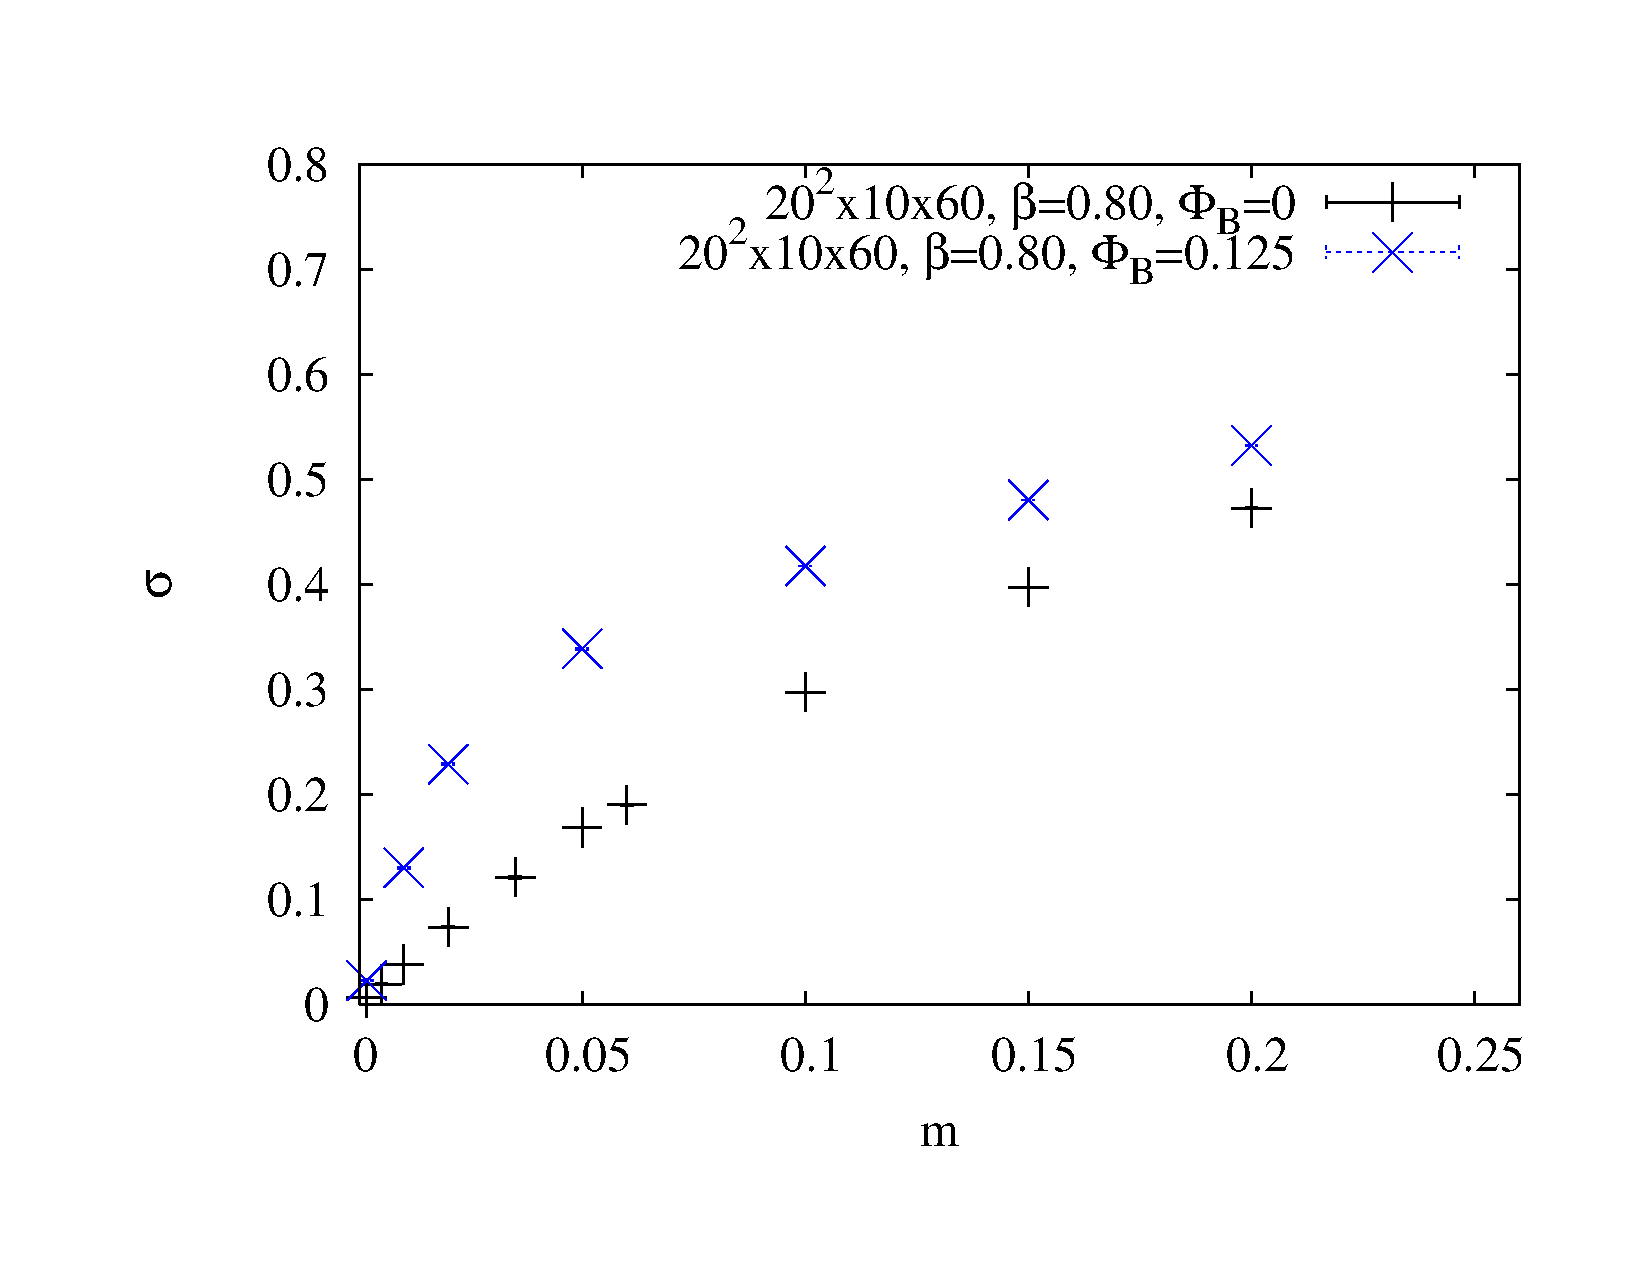
\includegraphics[height=8cm,width=8cm]{pbp_vs_m_compare_graphene_paper.pdf} \hspace{-1cm}
\caption{The chiral condensate $\sigma \equiv \vev{\Bpsi \Psi}$ as a function of the bare fermion mass at zero field (black points) and at magnetic flux $\Phi_B=0.125$ (blue points), where flux is measured in units of $a^2_s$. One can note that $\sigma$ vanishes with $m$ at zero field as well as at nonzero external field. The vanishing of the condensate in the presence of the magnetic field is argued to be a thermal effect. The error bars on each point are so small that they are not visible.}
\label{PBPComparison}
\end{figure}

\begin{figure}
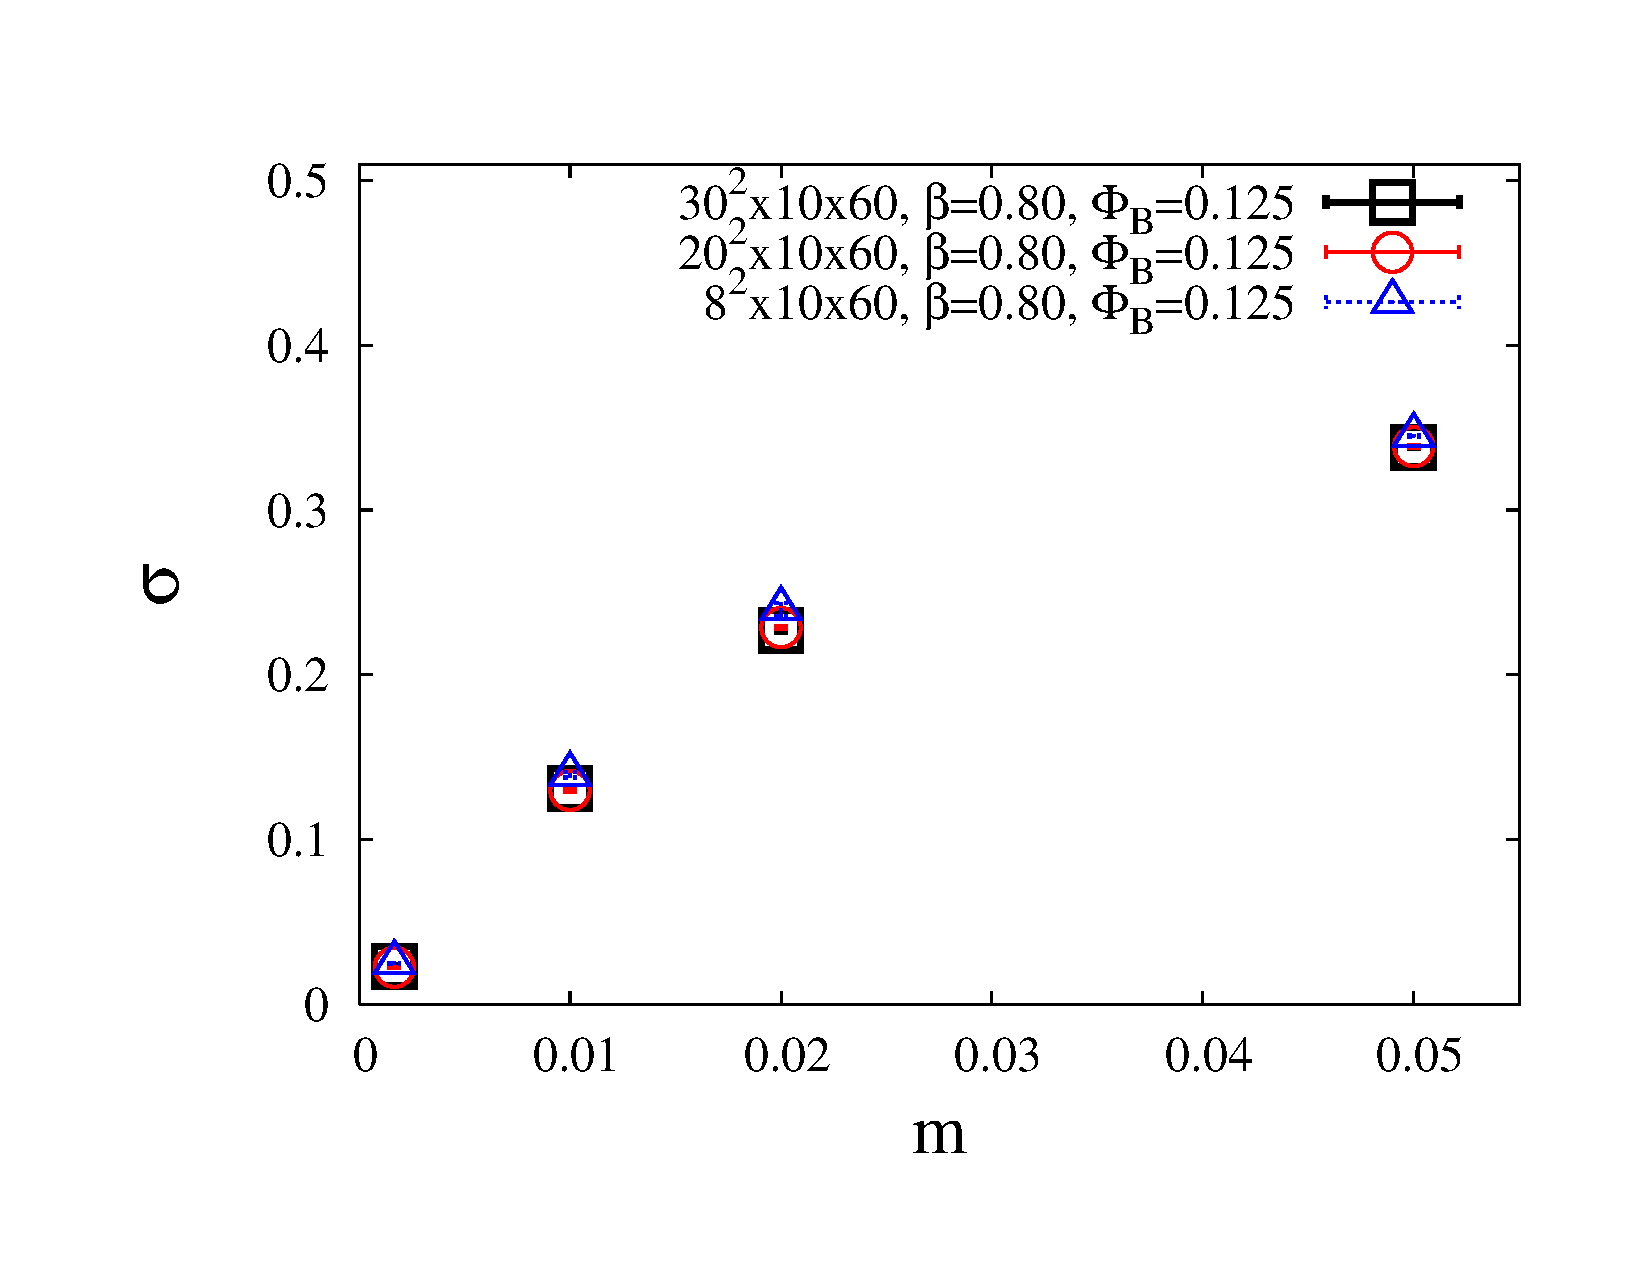
\includegraphics[height=8cm,width=8cm]{pbp_vs_m_PHI0125_volcompare_3_graphene_paper.pdf} \hspace{-1cm}
\caption{The chiral condensate $\sigma$ as a function of fermion mass with varying spatial volume $N^2_s$ for magnetic flux $\Phi_B=0.125$. The lattice volumes are listed in the form $N_s^2\times N_z \times N_{\tau}$ where the fermions live in the $xy$-plane and the gauge field is present throughout the entire volume.}
\label{PBPVolume}
\end{figure}

\begin{figure}
 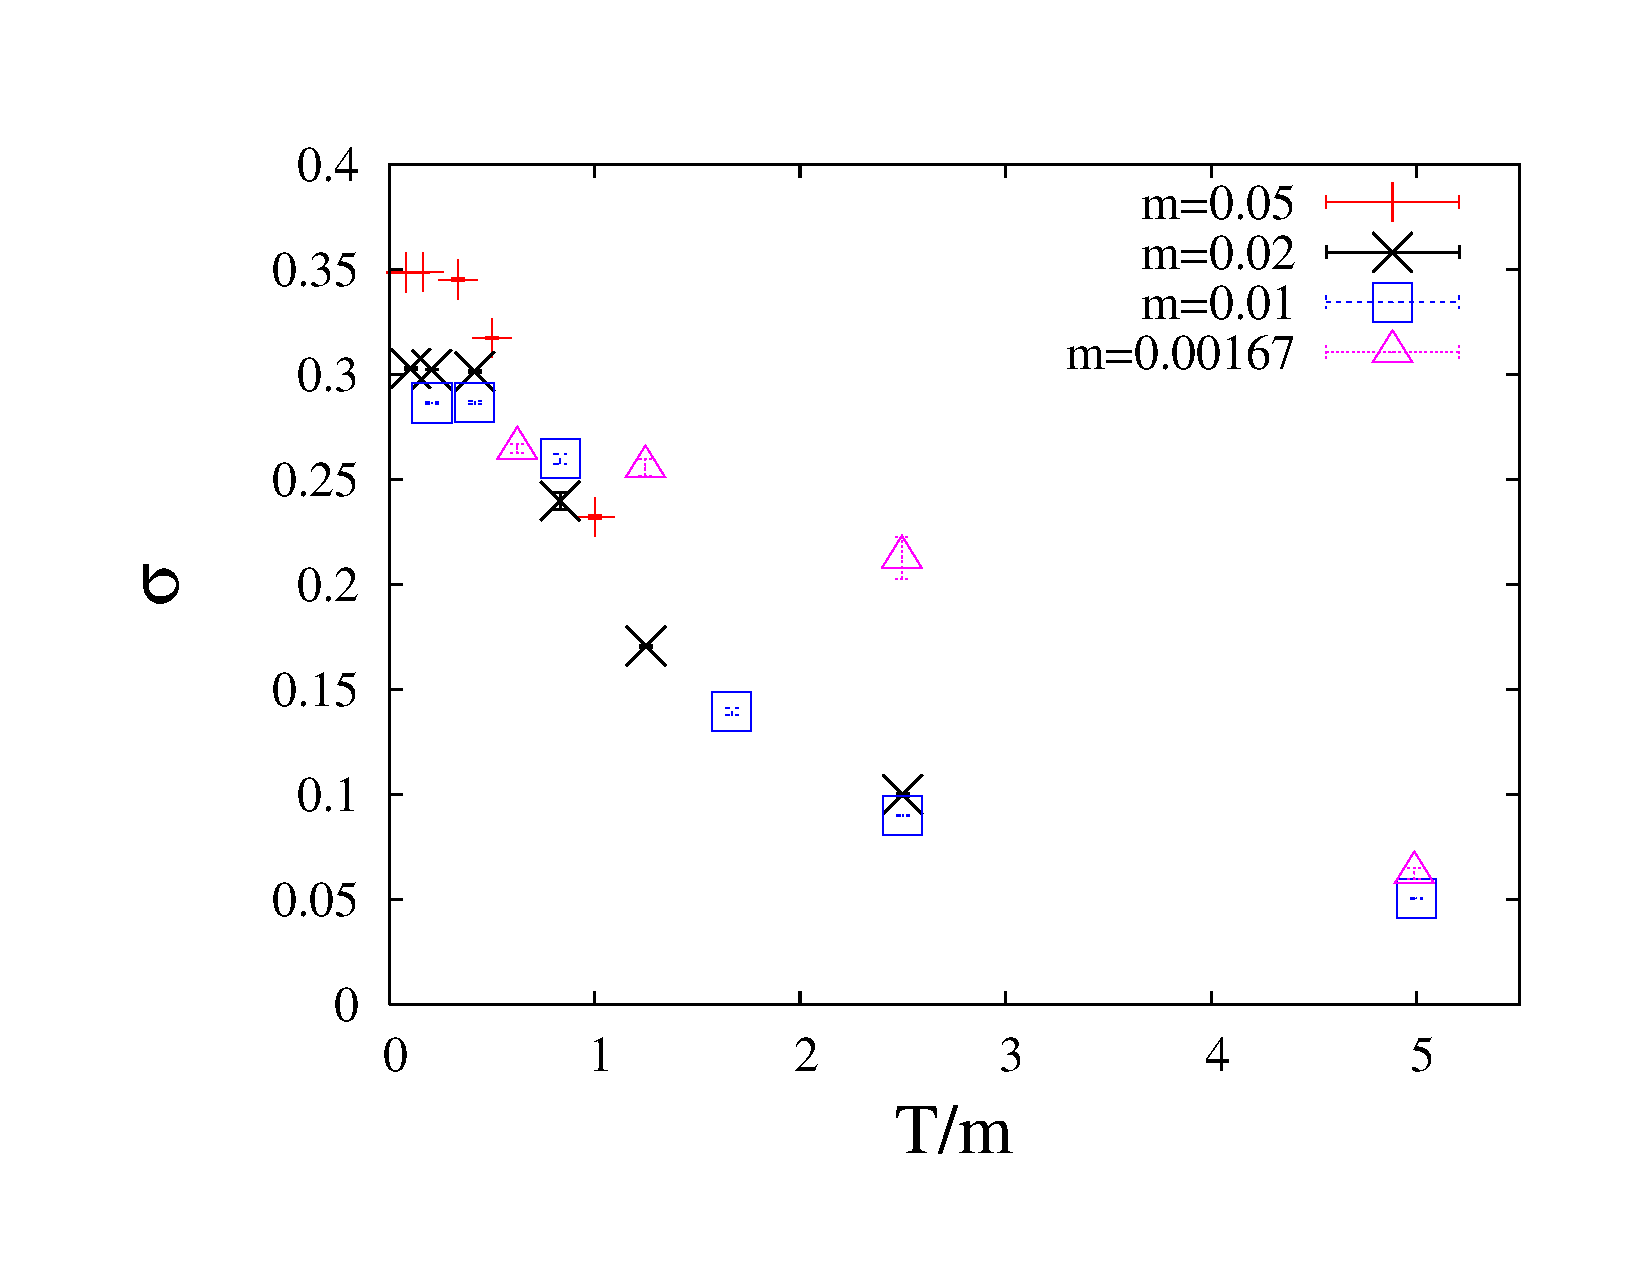
\includegraphics[height=8cm,width=8cm]{pbp_vs_TdivM_PHI0125_zoom_graphene_paper.pdf} \hspace{-1cm}
\caption{The chiral condensate $\sigma$ plotted as a function of $T/m$. One can see that at small values of $T/m$, the condensate increases and tends towards a nonzero value.}
\label{PBPvsTdivM}
\end{figure}

\begin{figure}
  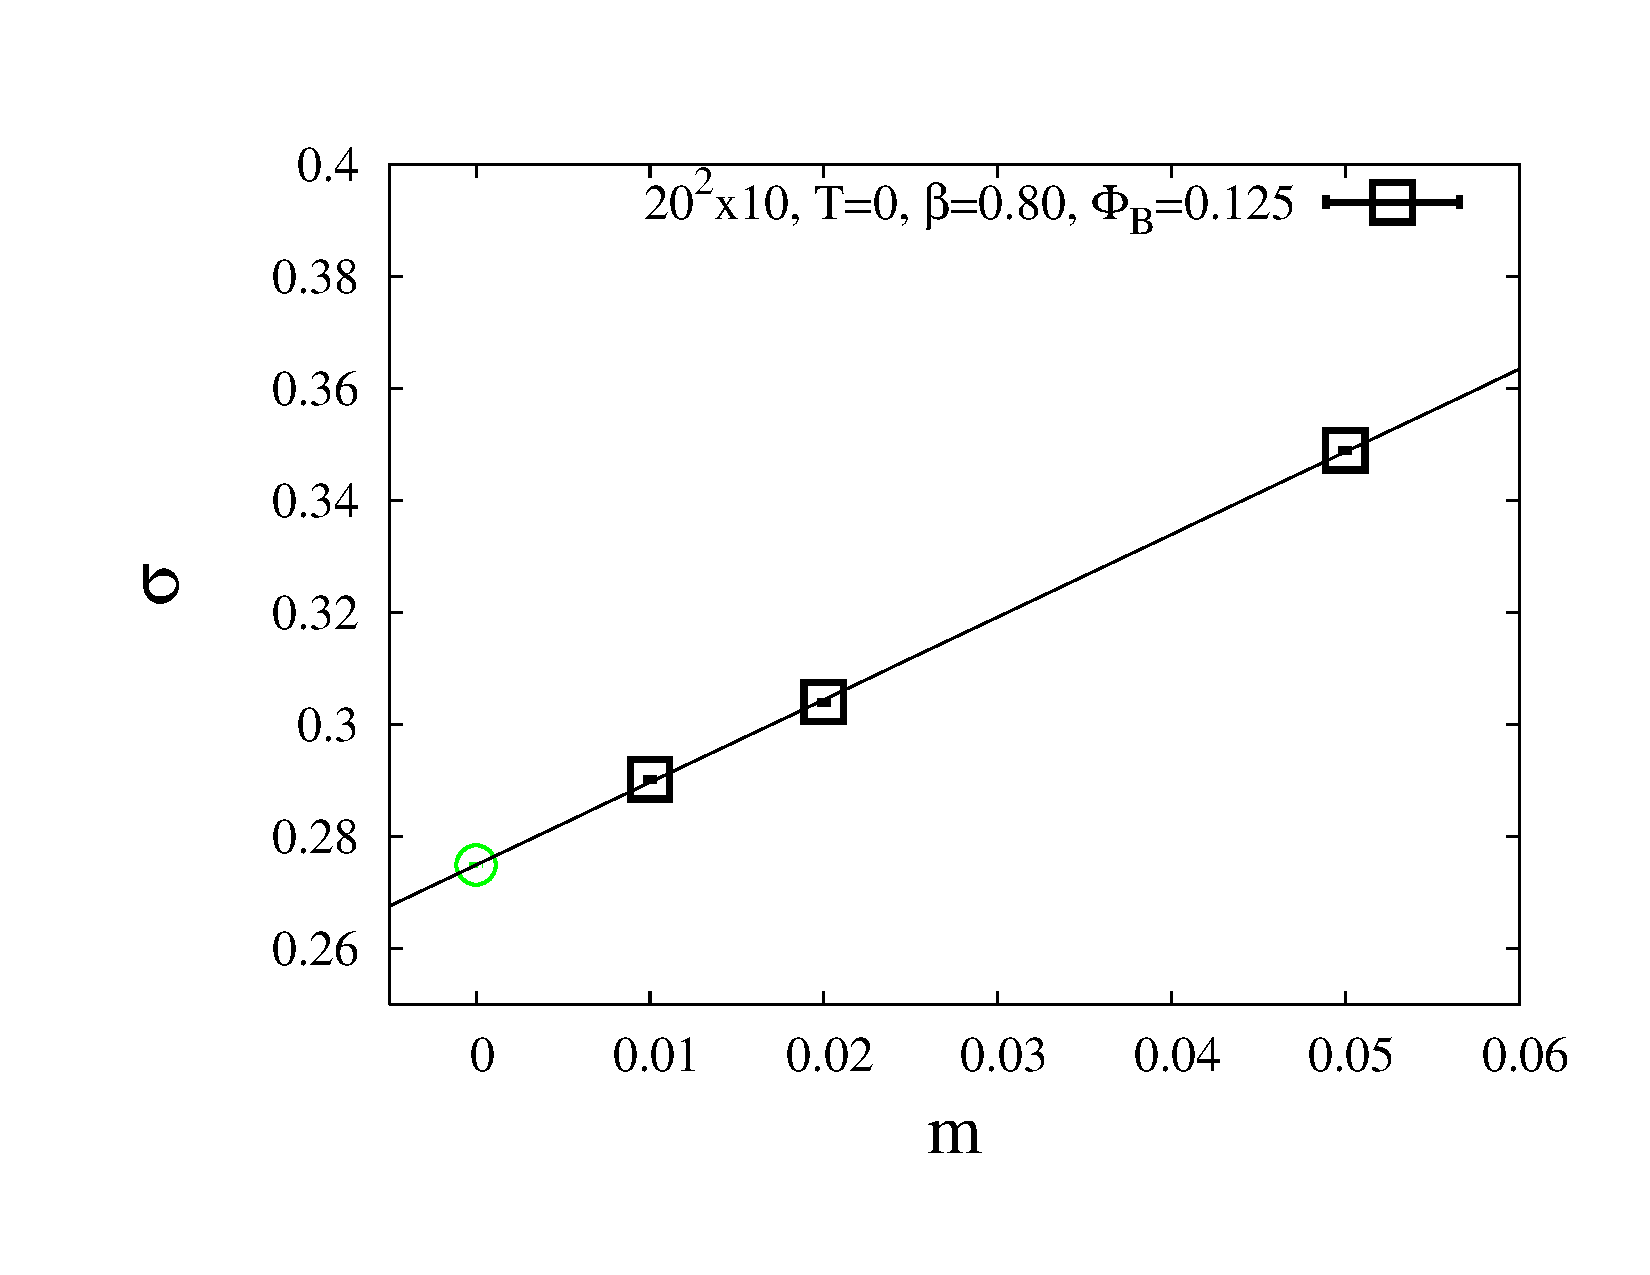
\includegraphics[height=8cm,width=8cm]{pbp_vs_m_zeroT_PHI0125_lin_graphene_paper.pdf} \hspace{-1cm}
\caption{Chiral limit of the chiral condensate $\sigma$ using the $T=0$ extrapolated points. The nonzero intercept indicates a finite value for the condensate in the chiral and zero temperature limits.}
\label{PBPzeroTChiral}
\end{figure}

\begin{figure}
 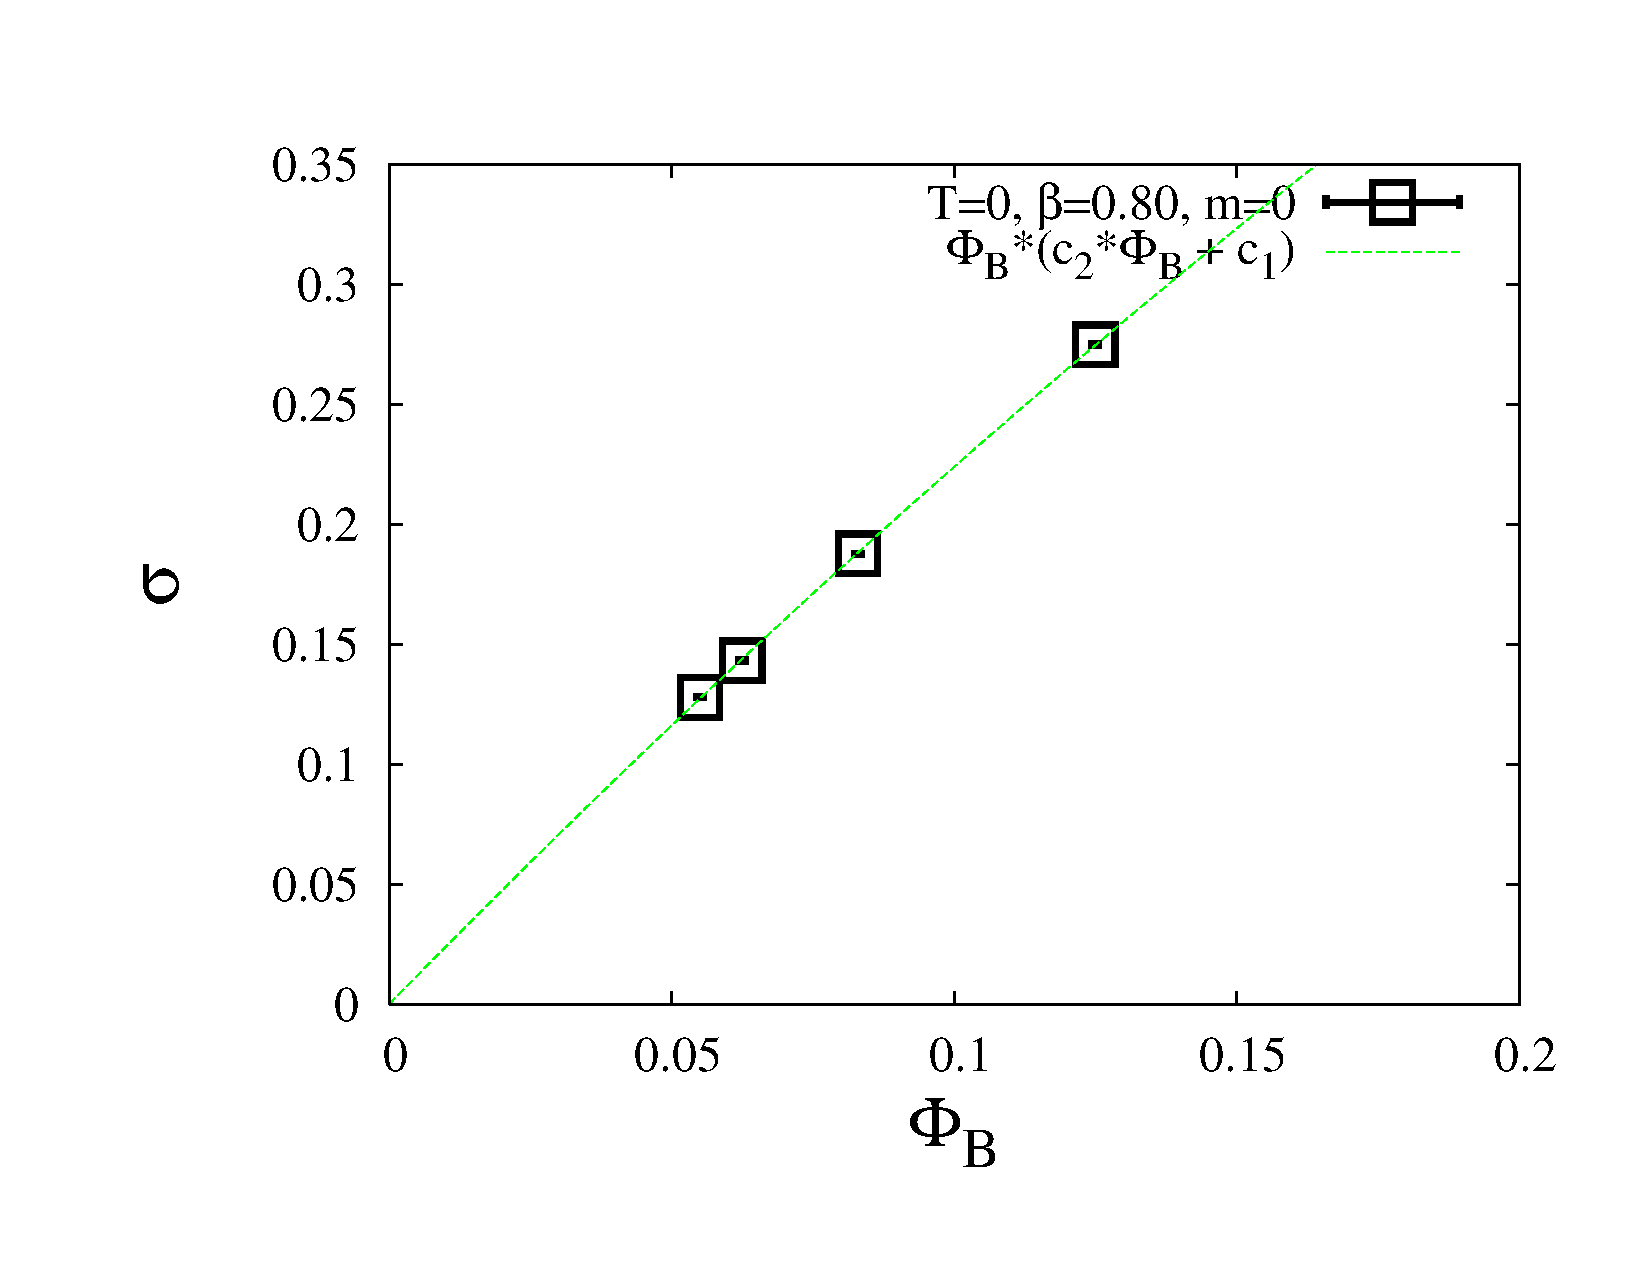
\includegraphics[height=8cm,width=8cm]{pbp_vs_PHI_NL_graphene_paper.pdf} \hspace{-1cm}
\caption{The chirally extrapolated, zero temperature values of the chiral condensate $\sigma$, plotted as a function of the magnetic flux,  $\Phi_B = eB/2\pi$. We have fit the data to a quadratic which passes through the origin. The fit has a $\chi^2/\text{d.o.f.} \approx 36/2$. } 
\label{PBPzeroTChiralvseB}
\end{figure}

\begin{figure}
 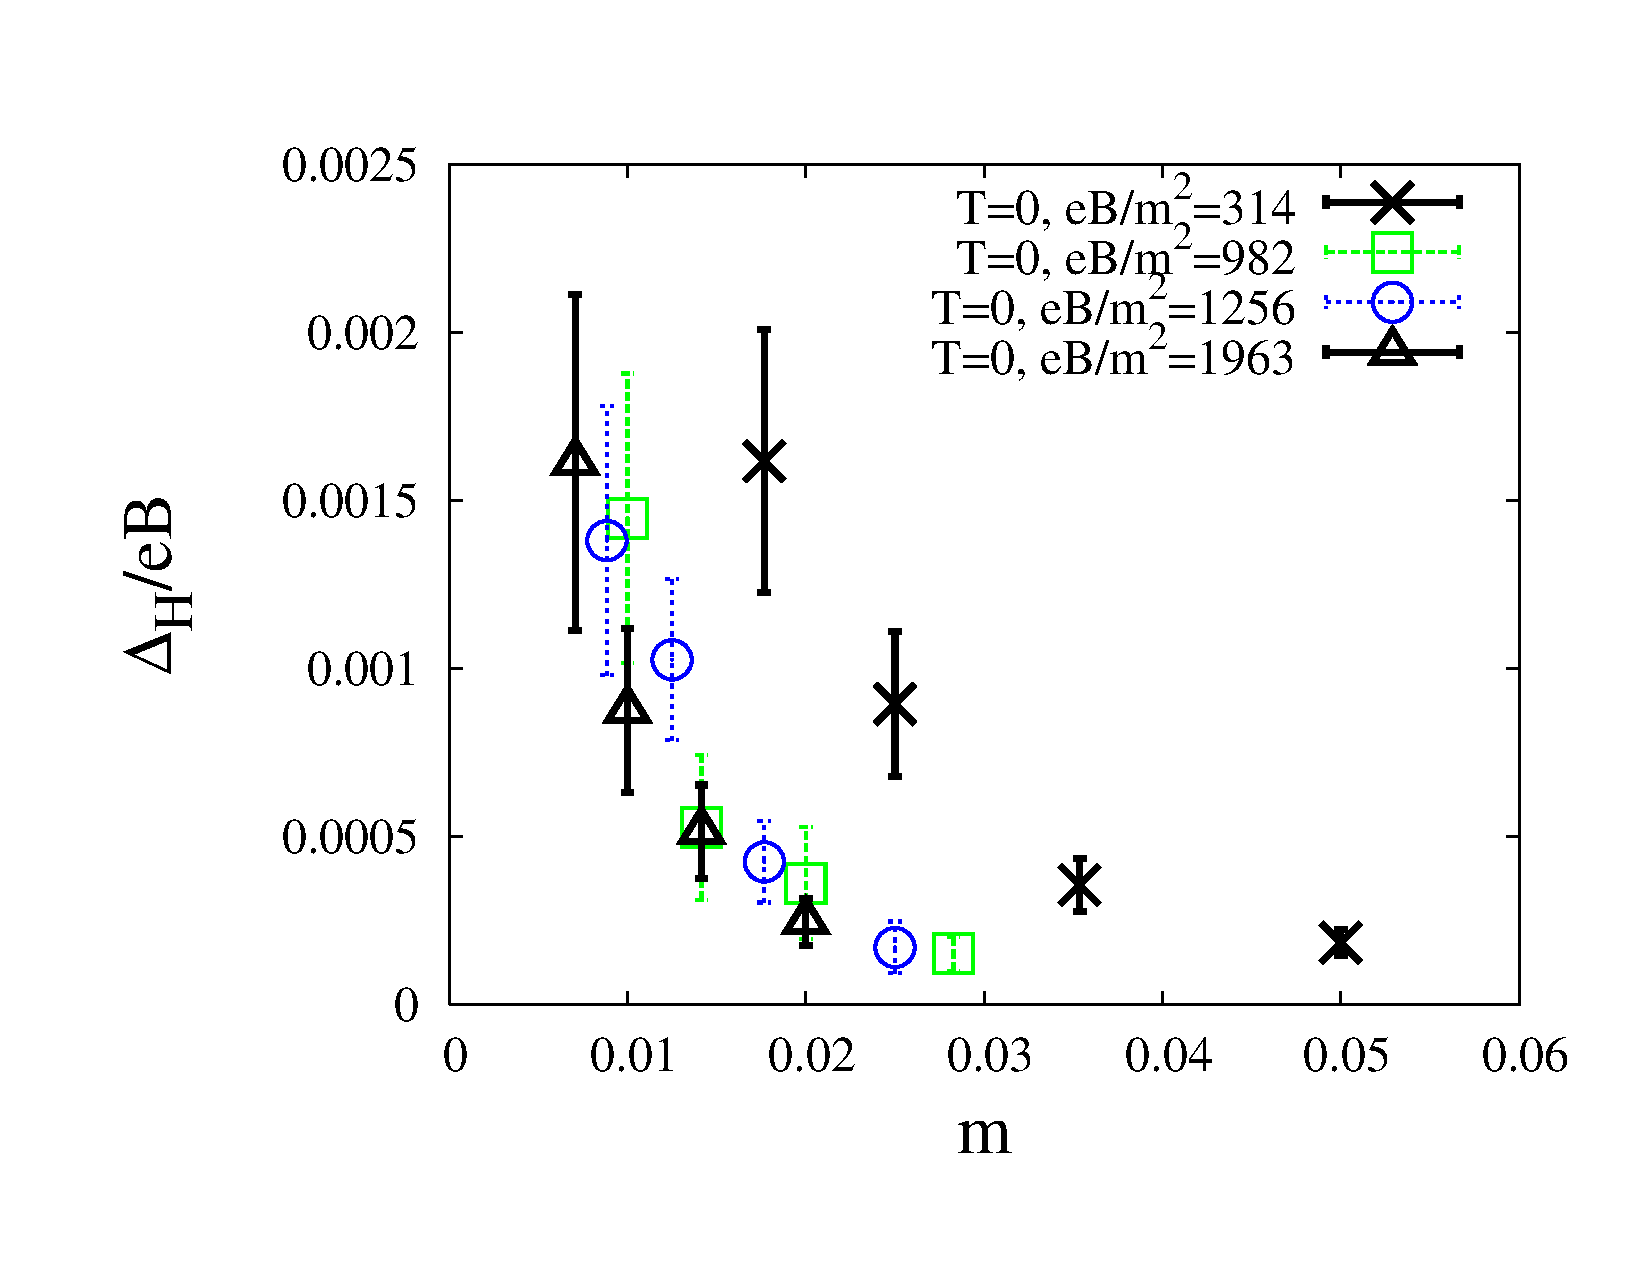
\includegraphics[height=8cm,width=8cm]{haldanediveB_vs_m_zeroT_graphene_paper.pdf} \hspace{-1cm}
\caption{The Haldane mass in units of magnetic flux, $\Delta_H/eB$, as a function of the lattice mass $\hat{m} = m a_t$. The behavior at small $\hat{m}$ indicates that
this quantity is UV divergent.}
\label{HaldanediveBvsm} 
\end{figure}

\begin{figure}
  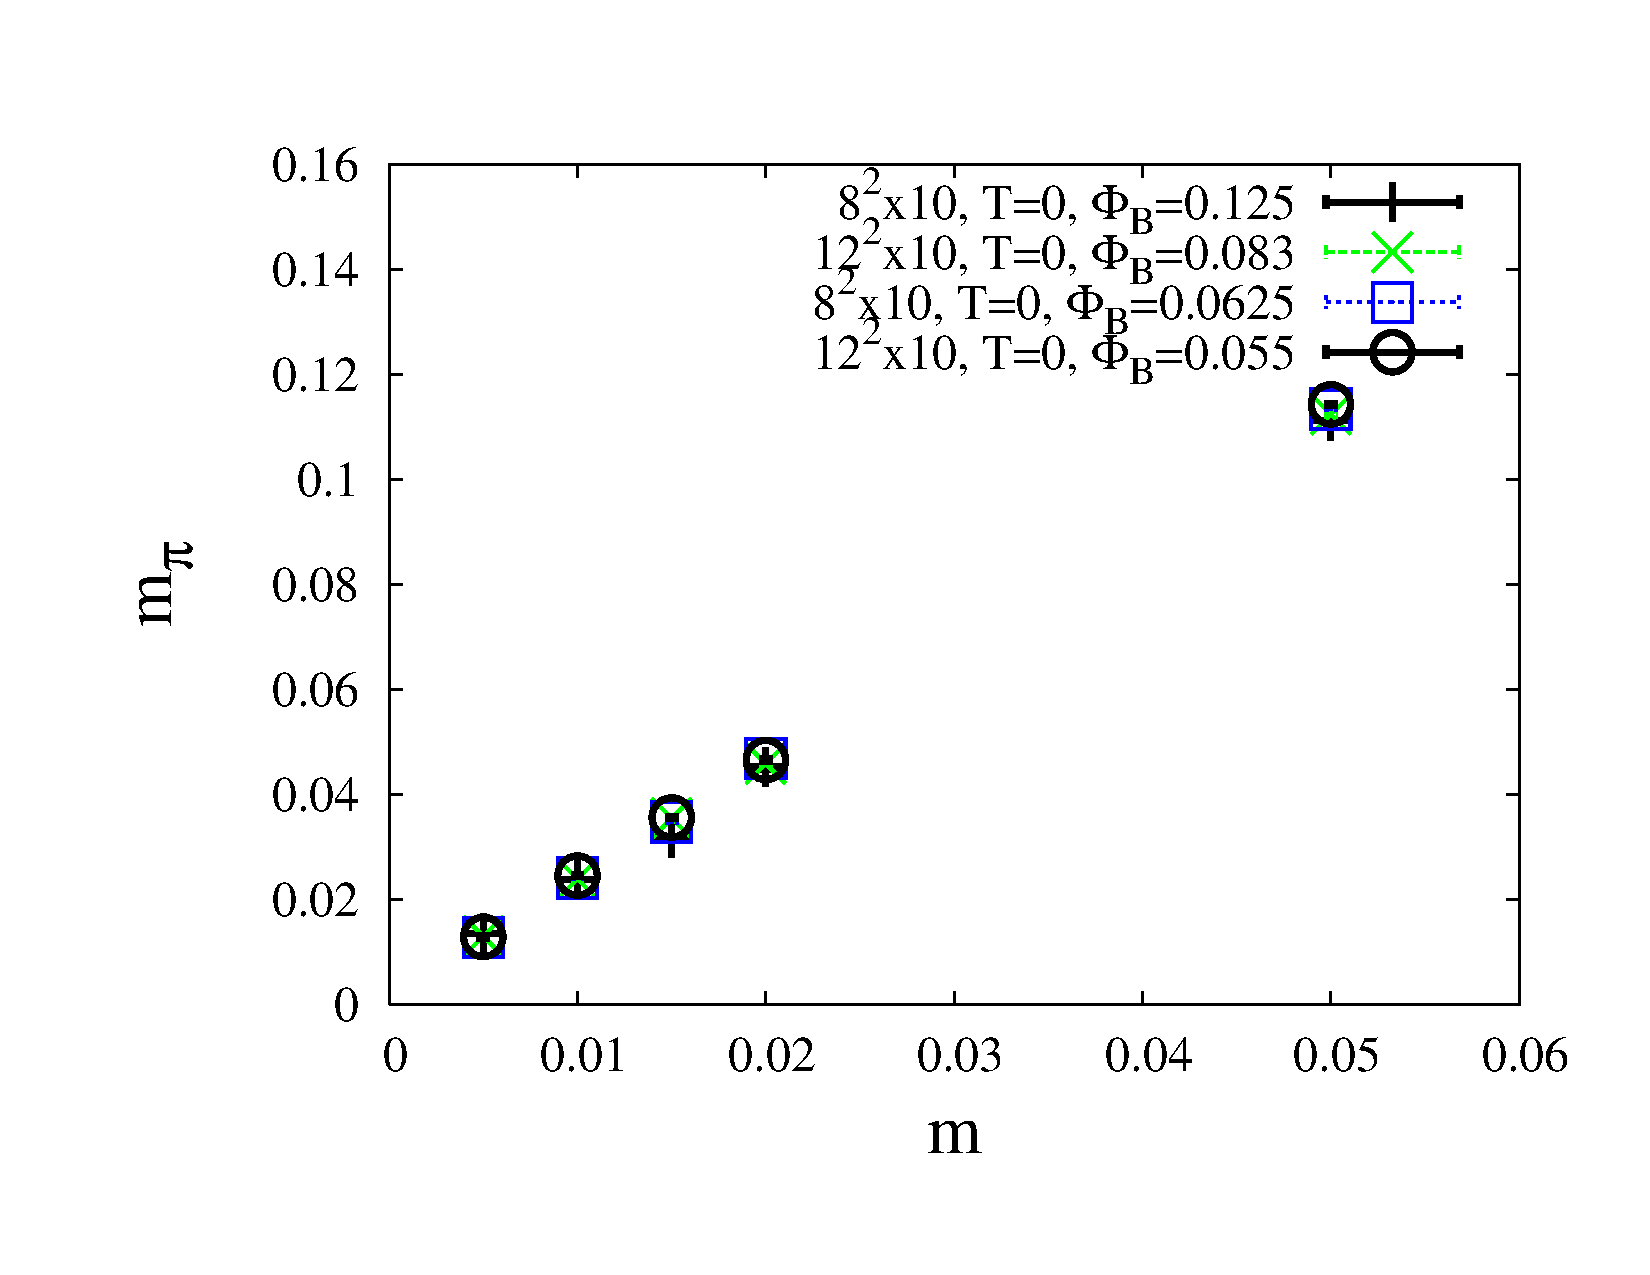
\includegraphics[height=8cm,width=8cm]{ps_mt_vs_m_2exp_graphene_paper.pdf} \hspace{-1cm}
\caption{The mass of the pseudoscalar bound state as a function of the bare fermion mass for all four magnetic fluxes.}
\label{MPSvsm}
\end{figure}

\begin{figure}
  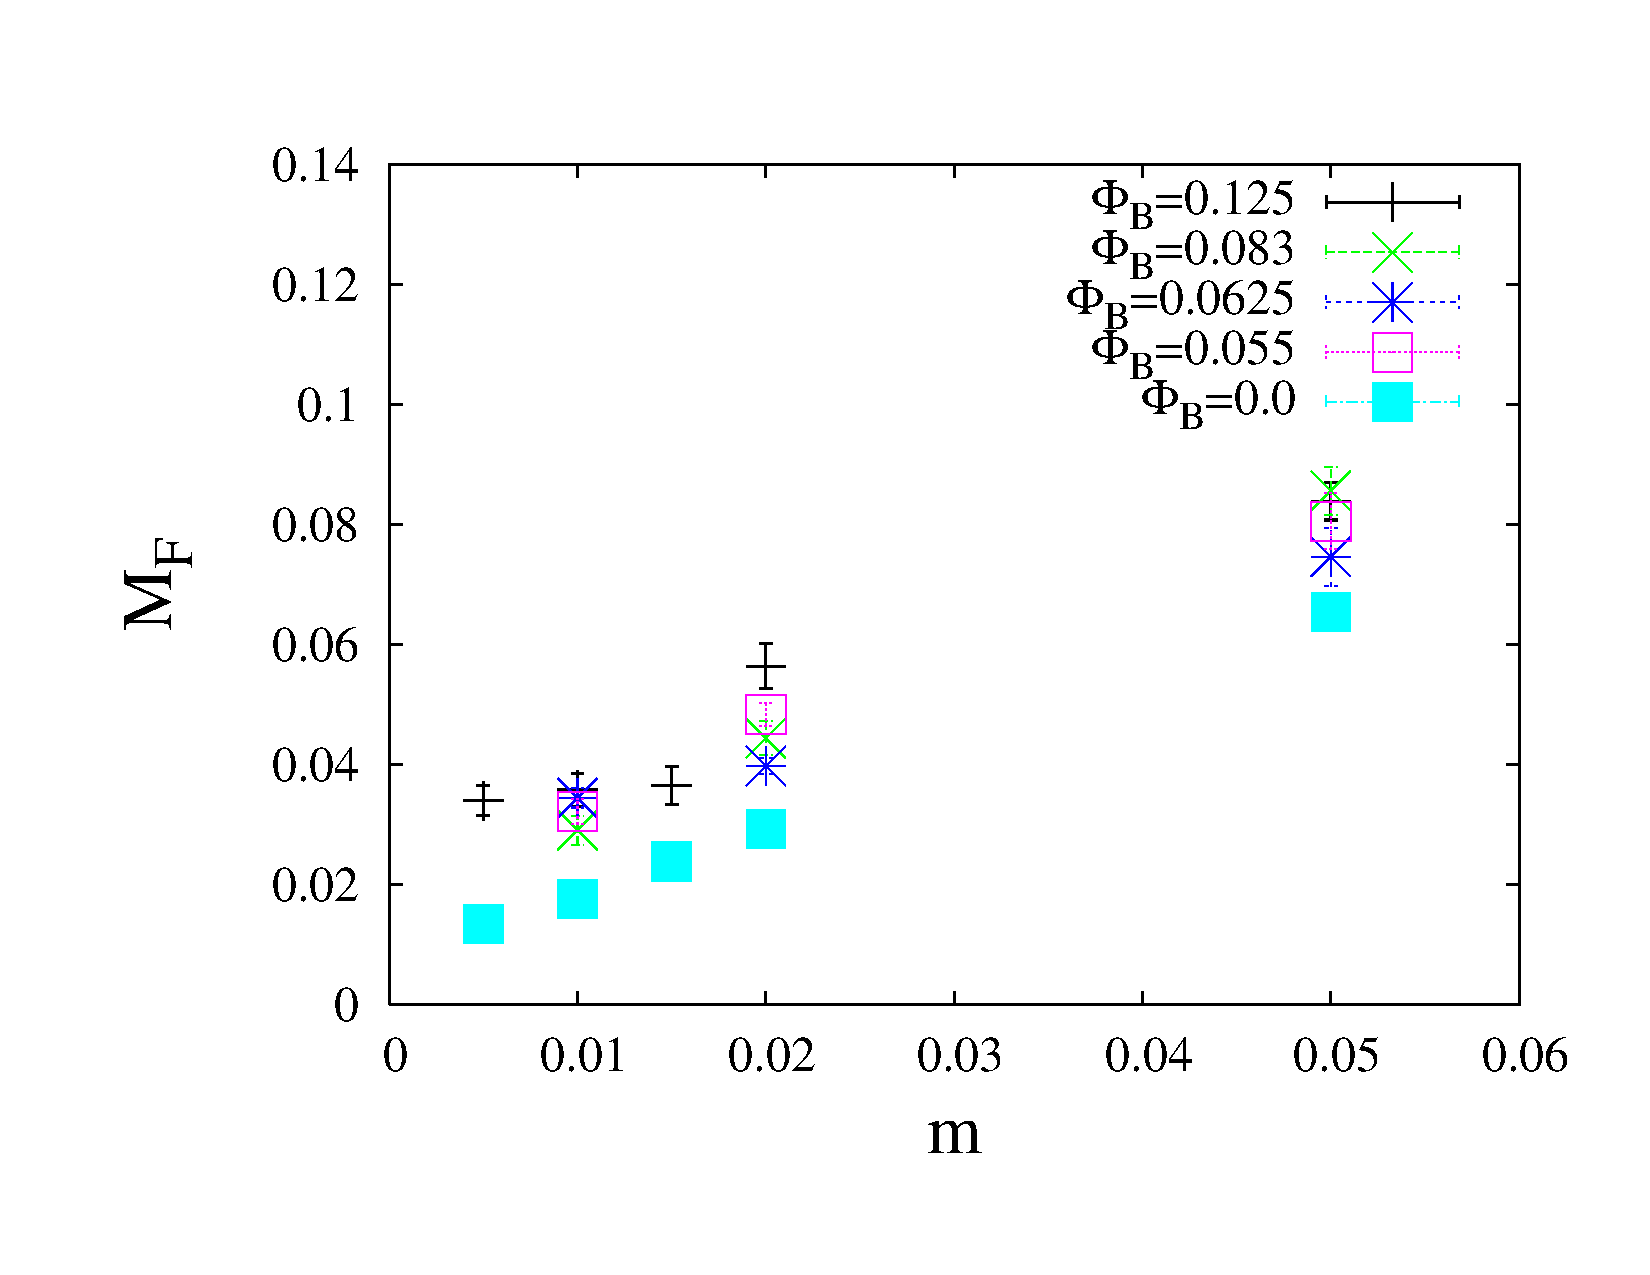
\includegraphics[height=8cm,width=8cm]{ferm_mt_vs_m_graphene_paper.pdf} \hspace{-1cm}
\caption{The pole of the fermion propagator as a function of the bare fermion mass for all four magnetic fluxes as well as at zero magnetic flux.}
\label{MFvsm}
\end{figure}

\section{\label{sec:Conclusion}Conclusion}

Through a thorough, fully non-perturbative study of the graphene EFT, we have shown the existence of spontaneous symmetry breaking due to an external magnetic field.
We have characterized the ground state of the system by performing a zero temperature extrapolation of our observables. Furthermore, ours is the first lattice study to present results 
for the Haldane mass. The evidence for a dynamically generated Dirac mass for the quasiparticle as well as the nonzero value for the chirally extrapolated, $T=0$ chiral condensate shows
that indeed, magnetic catalysis is occuring in the graphene EFT. Further studies of magnetic catalysis in the graphene EFT could address other questions, such as how the phase diagram presented in \cite{Polikarpov} changes as one varies the temperature.
This would necessarily involve a scan in $\beta$ which differs from our current study which was performed at fixed $\beta=0.80$. Another direction one could pursue would be to 
study the valley $\otimes$ sublattice and spin densities which are order parameters for Quantum Hall ferromagnetism (QHF). In a study of the Schwinger-Dyson gap equations, it was found that 
the appearance of the condensates associated with magnetic catalysis and those associated with QHF shared the same dynamical origin \cite{MiranskyGraphene2}.


\acknowledgements
This work was in part based on a variant of the MILC collaboration's public lattice gauge theory code. See {\bf http://physics.utah.edu/~detar/milc.html}.
Calculations were performed at the Center for High Performance Computing at the University of Utah, Fermi National Accelerator Laboratory, and the LOEWE-CSC high performance
computer of Johann Wolfgang Goethe-University Frankfurt. This work was granted access to the HPC resources of CINES and IDRIS under the allocations 2015-052271 and 2016-052271 made by GENCI.
The authors would like to acknowledge discussions with Maksim Ulybyshev. SZ would like to acknowledge discussions with Wolfgang Unger.
SZ would like to acknowledge the support of the Alexander von Humboldt foundation. CW and CD were supported by the US NSF grant PHY10-034278 and US DOE grant DOE DE-FC02-12ER41879.

\appendix
\section{\label{sec:SpinTasteAppendix}Spin-Taste Basis in $(2+1)$ dimensions}
In this appendix we discuss the spin taste basis in $(2+1)$ dimensions which has some differences with the more familiar $(3+1)$ dimensional case. 
The discussion follows that of \cite{Burkitt}. Starting from the one-component fields $\chi, \chib$ one performs a change of basis by introducing the following transformation
\beq
\label{SpinTasteTransfo2+1}
u^{\alpha a}(y) &=& \frac{1}{4\sqrt{2}} \sum_{\eta} \Gamma^{\alpha a}_{\eta} \chi_{\eta}(y), \\ \nn
d^{\alpha a}(y) &=& \frac{1}{4\sqrt{2}} \sum_{\eta} B^{\alpha a}_{\eta} \chi_{\eta}(y),
\eeq
where one has introduced the matrices 
\beq
\label{SpinTasteMatrices2+1}
\Gamma_{\eta} &\equiv& \sigma^{\eta_0}_0 \sigma^{\eta_1}_1 \sigma^{\eta_2}_2, \\ ~B_{\eta} &\equiv& \beta^{\eta_0}_0 \beta^{\eta_1}_1 \beta^{\eta_2}_2, ~\beta_{\mu}\equiv - \sigma_{\mu}.
\eeq
We note that one labels a lattice site by $n_{\mu} = 2y_{\mu} + \eta_{\mu}$, where $y_{\mu}$ is an integer that labels the corner of the cube, and $\eta_{\mu}=0,1$ labels the sites within a cube.
Using the identity $\tr{(\Gamma^{\dagger}_{\eta}\Gamma_{\eta'} + B^{\dagger}_{\eta}B_{\eta'})} = 4 \delta_{\eta \eta'}$, one can invert the relation in (\ref{SpinTasteTransfo2+1}) to obtain
\beq
\label{InverseSpinTasteTransfo2+1}
\chi_{\eta}(y) &=& \sqrt{2} \sum_{\alpha, a}(\Gamma^{* \alpha a}_{\eta} u^{\alpha a}(y) + B^{* \alpha a}_{\eta} d^{\alpha a}(y)), \\ \nn
\chib_{\eta}(y) &=& \sqrt{2} \sum_{\alpha, a}(\bar{u}^{\alpha a}(y)\Gamma^{\alpha a}_{\eta} + \bar{d}^{\alpha a}(y)B^{\alpha a}_{\eta}).
\eeq
One can then rewrite the action in the spin-taste basis. For example, the mass term becomes
\beq
&& a^3m\sum_{y,\eta} \chib_{\eta}(y) \chi_{\eta}(y) = \\ \nn && (2a)^3 \sum_y \left( \bar{u}(y)(\bm 1 \otimes \bm 1)u(y) + \bar{d}(y)(\bm 1 \otimes \bm 1)d(y) \right),
\eeq
where we have used the following identities
\beq
&& \sum_{\eta} \Gamma^{\alpha a}_{\eta} \Gamma^{*\beta b}_{\eta} = \sum_{\eta} B^{\alpha a}_{\eta} B^{*\beta b}_{\eta} = 4 \delta_{\alpha \beta} \delta_{a b}, \\
&& \sum_{\eta} \Gamma^{\alpha a}_{\eta} B^{*\beta b}_{\eta} = 0.
\eeq
To rewrite the kinetic term one first expresses the shifted field as 
\beq
&&\chi_{\eta + \hat{\mu}}(y) = \delta_{\eta_{\mu},0} \eta_{\mu}(\eta)\sqrt{2} \tr\bigg(\Gamma^{\dagger}_{\eta}\gamma_{\mu} u(y) + B^{\dagger}_{\eta}\beta_{\mu}d(y) \bigg) \\
\nn && + \delta_{\eta_{\mu},1} \eta_{\mu}(\eta)\sqrt{2} \tr\bigg(\Gamma^{\dagger}_{\eta} \gamma_{\mu}u(y+\hat{\mu}) + B^{\dagger}_{\eta}\beta_{\mu}d(y+\hat{\mu}) \bigg).
\eeq
A similar expression exists for the backward shifted field, $\chi_{\eta - \hat{\mu}}(y)$, and thus one arrives at the following form for the staggered action
\beq
\nn
S_{st} &=& (2a)^3 \sum_{y, \mu} \bigg\{ \bar{u}(y)(\sigma_{\mu} \otimes \bm 1)\partial_{\mu}u(y) + \bar{d}(y)(\beta_{\mu} \otimes \bm 1)\partial_{\mu}d(y) 
\\ \nn &+& a[\bar{u}(y)(\bm 1 \otimes \sigma^{T}_{\mu}) \partial^2_{\mu}d(y)  + \bar{d}(y)(\bm 1 \otimes \beta^{T}_{\mu}) \partial^2_{\mu}u(y)] \bigg\}
\\ &+& (2a)^3 m \sum_y [\bar{u}(y)(\bm 1 \otimes \bm 1)u(y) + \bar{d}(y)(\bm 1 \otimes \bm 1)d(y)],
\eeq
where $\sigma^{T}_{\mu}$ refers to the transpose and derivative operators now act on a lattice of spacing $2a$. One can now define a four-component Dirac spinor as follows
\beq
\label{SpinTastePsi}
\Psi(y) = \left( \begin{array}{c} u(y) \\ d(y) \end{array} \right).
\eeq
Using the reducible set of gamma matrices in (\ref{Gammas1}) and (\ref{Gammas2}) one can write the action in the following compact form
\beq
\label{SpinTasteAction2+1}
S_{st} &=& (2a)^3 \sum_{y, \mu} \bigg\{ \bar{\Psi}(y)(\gamma_{\mu} \otimes \bm 1)\partial_{\mu}\Psi(y) \\ \nn &+& a\bar{\Psi}(y)(\tilde{\gamma}_5 \otimes \gamma^{T}_{\mu}) \partial^2_{\mu}\Psi(y) \bigg\}
\\ \nn &+& (2a)^3 m \sum_y \bar{\Psi}(y)(\bm 1 \otimes \bm 1)\Psi(y).
\eeq
One sees from (\ref{SpinTasteAction2+1}) that the second derivative term, which is suppressed by a factor of the lattice spacing, is not invariant under a rotation in taste space.

The residual symmetry of the staggered lattice action is $U(1) \otimes U(1)_{\epsilon}$. The form of these symmetries on the one-component fields is as follows
\beq
\nn
&& \chi(x) \to \exp(i\alpha) \chi(x), \\  &&\bar{\chi}(x) \to \bar{\chi}(x) \exp(-i\alpha), \\ \nn
&& \chi(x) \to \exp(i\beta \epsilon(x)) \chi(x), \\ && \bar{\chi}(x) \to \bar{\chi}(x) \exp(i\beta \epsilon(x)),
\eeq
where $\epsilon(x) \equiv (-1)^{x_0 + x_1 + x_2}$. In terms of the fields $u$ and $d$, these transformations become
\beq
\nn
&&\left(\begin{array}{c} u \\d \end{array}\right) \to \exp(i\alpha) \left(\begin{array}{c} u \\d \end{array}\right), \\ && \left(\begin{array}{cc} \bar{u} & \bar{d} \end{array}\right) \to
 \left(\begin{array}{cc} \bar{u} & \bar{d} \end{array}\right) \exp(-i\alpha), \\
\label{U1}
\nn
&& \left(\begin{array}{c} u \\d \end{array}\right) \to \left(\begin{array}{cc} \cos(\beta) & i\sin(\beta) \\ i\sin(\beta) & \cos(\beta) \end{array}\right) \left(\begin{array}{c} u \\d \end{array}\right), \\ 
&& \left(\begin{array}{cc} \bar{u} & \bar{d} \end{array}\right) \to  \left(\begin{array}{cc} \bar{u} & \bar{d} \end{array}\right) \left(\begin{array}{cc} \cos(\beta) & i\sin(\beta) \\ i\sin(\beta) & \cos(\beta) \end{array}\right).
\eeq
Thus, one can see that the formation of the condensate $\vev{\chib \chi}$ spontaneously breaks the $U(1)_{\epsilon}$ symmetry and leads to the appearance of a single NG boson.

\section{\label{sec:FermionAppendix}Fermion Bilinears}
In our study we are looking for spontaneous symmetry breaking in the presence of an external magnetic field. Typically, this will involve the breaking of the $SU(2)_{\sigma}$ symmetry, where
$SU(2)_{\sigma}$ is the largest non-abelian subgroup of $U(2)_{\sigma}$, described in (\ref{U2Generators}). In this appendix, we list the expressions for the various bilinear operators in terms of the degrees of freedom on the hexagonal lattice
as well as their representation in terms of staggered lattice fermions.

We first introduce the Dirac mass term
\beq
\label{DiracMass}
\tilde{\Delta}_{\sigma} \Bpsi P_{\sigma} \Psi = \tilde{\Delta}_{\sigma} \Psi^{\dagger} \gamma_0 P_{\sigma} \Psi,
\eeq
which is a triplet with respect to spin and breaks $SU(2)_{\sigma}$ down to $U(1)_{\sigma}$ with the generator $\tilde{\gamma}_{4,5} \otimes P_{\sigma}$. The corresponding order parameter for this term is $\vev{\Bpsi P_{\sigma} \Psi}$ and written in terms
of Bloch components it can be expressed as
\beq
\label{DiracMassComponents}
\nn
&\tilde{\Delta}_{\sigma}:& \quad \psi^{\dagger}_{\kappa A \sigma} \psi_{\kappa A \sigma} - \psi^{\dagger}_{\kappa B \sigma}\psi_{\kappa B \sigma} \\
&+& \psi^{\dagger}_{\kappa' A \sigma}\psi_{\kappa' A \sigma} - \psi^{\dagger}_{\kappa' B \sigma} \psi_{\kappa' B \sigma}.
\eeq
One can interpret a nonzero value for this order parameter as an imbalance of charge between the two sublattices, A and B, corresponding to a charge density wave (CDW).

The Haldane mass term is given by
\beq
\label{HaldaneMass}
\Delta_{\sigma} \Bpsi \tilde{\gamma}_{4,5} P_{\sigma} \Psi = \Delta_{\sigma} \Psi^{\dagger} \gamma_0 \tilde{\gamma}_{4,5} P_{\sigma} \Psi,
\eeq
which is a singlet with respect to spin but is odd under time-reversal. The order parameter for the Haldane mass is $\vev{\Bpsi \tilde{\gamma}_{4,5} P_{\sigma} \Psi}$, and its expression 
in terms of Bloch components is given by
\beq
\label{HaldaneMassComponents}
\nn
&\Delta_{\sigma}:& \quad \psi^{\dagger}_{\kappa A \sigma} \psi_{\kappa A \sigma} - \psi^{\dagger}_{\kappa' A \sigma}\psi_{\kappa' A \sigma} \\
&-& \psi^{\dagger}_{\kappa B \sigma}\psi_{\kappa B \sigma} + \psi^{\dagger}_{\kappa' B \sigma} \psi_{\kappa' B \sigma}.
\eeq
Thus, this order parameter can be seen to represent a charge imbalance between the two valleys, $\kappa$ and $\kappa'$.
To discuss the properties of (\ref{HaldaneMass}) under time-reversal, we introduce the Hamiltonian of the low-energy theory
\beq
\label{EFTHamiltonian}
\mathcal{H}(\vec{k}) = \hbar v_F \tau_0 \otimes \vec{\sigma} \cdot \vec{k},
\eeq
where $\tau_0$ is a two-dimensional unit matrix in valley space which is tensored with the two-dimensional sublattice space. 
Time-reversal invariance imposes the following restriction on the states as well as the valley Hamiltonians themselves
\beq
\label{TReversalStates}
T \psi_{\kappa (A,B)} &=& \psi^{*}_{\kappa (A,B)} = \psi_{\kappa' (A,B)}, \\
\label{TReversalHamiltonians}
T\mathcal{H}_{\kappa} T^{-1} &=& \mathcal{H}^{*}_{\kappa'}.
\eeq
The relation in (\ref{TReversalStates}) can be seen by shown by inspecting the explicit form of the valley Hamiltonian eigenstates
\beq
\psi^{\kappa}_{e.h.} = \frac{1}{\sqrt{2}} \left(\begin{array}{cc} e^{-i\phi_{\vec{k}}/2}  \\ \pm  e^{i\phi_{\vec{k}}/2} \end{array}\right), \\ 
\psi^{\kappa'}_{e.h.} = \frac{1}{\sqrt{2}} \left(\begin{array}{cc} e^{i\phi_{\vec{k}}/2}  \\ \pm  e^{-i\phi_{\vec{k}}/2} \end{array}\right), 
\eeq
where the $\pm$ refers to electron and hole states respectively, and $\phi_{\vec{k}} \equiv \tan^{-1}\left(\frac{k_y}{k_x}\right)$ describes the orientation of the vector $\vec{k}$ in the plane. 
Applying the transformation in (\ref{TReversalHamiltonians}) to (\ref{HaldaneMass}), one can verify that this term is odd under time-reversal.

On the lattice, we must calculate the relevant condensates in the language of staggered lattice fermions. In $(2+1)$ dimensions, a bilinear in the spin-taste basis takes the form
\beq
\label{SpinTasteBilinear}
\Bpsi(y)\left( \Gamma_S \otimes \Gamma_T \right) \Psi(y),
\eeq
where the four-component Dirac spinor $\Psi$ is defined in (\ref{DiracSpinorBasis}). From the above discussion, one can see that the four-dimensional spin space can be mapped to the 
four-dimensional sublattice $\otimes$ valley subspace and the two-dimensional taste space can be mapped to the two-dimensional spin of the electron. 

The Dirac mass is the usual staggered mass ($\Gamma_S = \Gamma_T = \bm 1$), and takes the form 
\beq
\label{Condensate}
\nn
\Bpsi(y) \left( \bm 1 \otimes \bm 1 \right) \Psi(y) &=& \bar{u}(y) \left( \bm 1 \otimes \bm 1 \right) u(y) \\ \nn
 &+& \bar{d}(y) \left( \bm 1 \otimes \bm 1 \right) d(y) \\
&=& \frac{1}{8} \sum_{\eta} \chib_{\eta}(y) \chi_{\eta}(y),
\eeq
where we have used the identity $\tr{(\Gamma^{\dagger}_{\eta}\Gamma_{\eta'} + B^{\dagger}_{\eta}B_{\eta'})} = 4 \delta_{\eta \eta'}$. We note that in our lattice calculations, we do not isolate the 
individual spin contributions to the condensates ($\Gamma_T = \bm 1$ i.e. $P_{\sigma} \to \bm 1$). 

The Haldane mass in the spin-taste basis takes the following form
\beq
\label{Haldane1}
\nn
\Bpsi(y) \left( \tilde{\gamma}_{4,5} \otimes \bm 1 \right) \Psi(y) &=& \bar{u}(y) \left( \bm 1 \otimes \bm 1 \right) u(y) \\ \nn
&-& \bar{d}(y) \left( \bm 1 \otimes \bm 1 \right) d(y) \\
&=& \frac{i}{8} \sum_{\eta_{\mu} \neq \eta'_{\mu}} \bar{\chi}_{\eta}(y) \chi_{\eta'}(y),
\eeq
where we have employed the identity
\beq
\tr \left[ \Gamma^{\dagger}_{\eta}\Gamma_{\eta'} - B^{\dagger}_{\eta}B_{\eta'} \right] = \left\{ \begin{array}{ll} 4i, &  \eta_{\mu} \neq \eta'_{\mu}, \forall \mu \\
                                                                                             0, & \mbox{otherwise}
                                                                                            \end{array} \right..
\eeq
Thus the Haldane mass involves a bilinear with the fields residing on diagonally opposite sites within the cube. This operator is left invariant by the staggered lattice action's $U(1)_{\epsilon}$ symmetry.
% This sample document demonstrates proper use of REV\TeX~4 (and
% \LaTeXe) in mansucripts prepared for submission to APS
% journals. Further information can be found in the REV\TeX~4
% documentation included in the distribution or available at
% \url{http://publish.aps.org/revtex4/}.
% 
% When commands are referred to in this example file, they are always
% shown with their required arguments, using normal \TeX{} format. In
% this format, \verb+#1+, \verb+#2+, etc. stand for required
% author-supplied arguments to commands. For example, in
% \verb+\section{#1}+ the \verb+#1+ stands for the title text of the
% author's section heading, and in \verb+\title{#1}+ the \verb+#1+
% stands for the title text of the paper.
% 
% Line breaks in section headings at all levels can be introduced using
% \textbackslash\textbackslash. A blank input line tells \TeX\ that the
% paragraph has ended. Note that top-level section headings are
% automatically uppercased. If a specific letter or word should appear in
% lowercase instead, you must escape it using \verb+\lowercase{#1}+ as
% in the word ``via'' above.
% 
% %\subsection{\label{sec:level2}Second-level heading: Formatting}
% % subsections are not used for PRL papers
% 
% This file may be formatted in both the \texttt{preprint} and
% \texttt{twocolumn} styles. \texttt{twocolumn} format may be used to
% mimic final journal output. Either format may be used for submission
% purposes; however, for peer review and production, APS will format the
% article using the \texttt{preprint} class option. Hence, it is
% essential that authors check that their manuscripts format acceptably
% under \texttt{preprint}. Manuscripts submitted to APS that do not
% format correctly under the \texttt{preprint} option may be delayed in
% both the editorial and production processes.
% 
% The \texttt{widetext} environment will make the text the width of the
% full page.  The width-changing commands only take effect in \texttt{twocolumn}
% formatting. It has no effect if \texttt{preprint} formatting is chosen
% instead.
% 
% To cite bibliography entries, use the \verb+\cite{#1}+ command. Most
% journal styles will display the corresponding number(s) in square
% brackets: \cite{d0det}. To avoid the square brackets, use
% \verb+\onlinecite{#1}+: Refs.~\onlinecite{d0det} and
% \onlinecite{geant,pythia}. REV\TeX\ ``collapses'' lists of
% consecutive reference numbers where possible. We now cite everyone
% together \cite{geant, pythia, cteq}, and once again
% (Refs.~\onlinecite{geant, pythia, cteq}). Note that the references
% were also sorted into the correct numerical order as well.
% 
% Footnotes are produced using the \verb+\footnote{#1}+ command. Most
% APS journal styles put footnotes into the bibliography. REV\TeX~4 does
% this as well, but instead of interleaving the footnotes with the
% references, they are listed at the end of the references. Because the correct
% numbering of the footnotes must occur after the numbering of the
% references, an extra pass of \LaTeX\ is required in order to get the
% numbering correct.
% 
% 
% Inline math may be typeset using the \verb+$+ delimiters. Bold math
% symbols may be achieved using the \verb+bm+ package and the
% \verb+\bm{#1}+ command it supplies. For instance, a bold $\alpha$ can
% be typeset as \verb+$\bm{\alpha}$+ giving $\bm{\alpha}$. Fraktur and
% Blackboard (or open face or double struck) characters should be
% typeset using the \verb+\mathfrak{#1}+ and \verb+\mathbb{#1}+ commands
% respectively. Both are supplied by the \texttt{amssymb} package. For
% example, \verb+$\mathbb{R}$+ gives $\mathbb{R}$ and
% \verb+$\mathfrak{G}$+ gives $\mathfrak{G}$
% 
% In \LaTeX\ there are many different ways to display equations, and a
% few preferred ways are noted below. Displayed math will center by
% default. Use the class option \verb+fleqn+ to flush equations left.
% 
% Below we have numbered single-line equations; this is the most common
% type of equation in \textit{Physical Review}:
% \begin{eqnarray}
% \chi_+(p)\alt{\bf [}2|{\bf p}|(|{\bf p}|+p_z){\bf ]}^{-1/2}
% \left(
% \begin{array}{c}
% |{\bf p}|+p_z\\
% px+ip_y
% \end{array}\right)\;,
% \\
% \left\{%
%  \openone234567890abc123\alpha\beta\gamma\delta1234556\alpha\beta
%  \frac{1\sum^{a}_{b}}{A^2}%
% \right\}%
% \label{eq:one}.
% \end{eqnarray}
% Note the open one in Eq.~(\ref{eq:one}).
% 
% Not all numbered equations will fit within a narrow column this
% way. The equation number will move down automatically if it cannot fit
% on the same line with a one-line equation:
% \begin{equation}
% \left\{
%  ab12345678abc123456abcdef\alpha\beta\gamma\delta1234556\alpha\beta
%  \frac{1\sum^{a}_{b}}{A^2}%
% \right\}.
% \end{equation}
% 
% When the \verb+\label{#1}+ command is used [cf. input for
% Eq.~(\ref{eq:one})], the equation can be referred to in text without
% knowing the equation number that \TeX\ will assign to it. Just
% use \verb+\ref{#1}+, where \verb+#1+ is the same name that used in
% the \verb+\label{#1}+ command.
% 
% Unnumbered single-line equations can be typeset
% using the \verb+\[+, \verb+\]+ format:
% \[g^+g^+ \rightarrow g^+g^+g^+g^+ \dots ~,~~q^+q^+\rightarrow
% q^+g^+g^+ \dots ~. \]
% 
% 
% Figures may be inserted by using either the \texttt{graphics} or
% \texttt{graphicx} packages. These packages both define the
% \verb+\includegraphics{#1}+ command, but they differ in how optional
% arguments for specifying the orientation, scaling, and translation of the
% figure. %Fig.~\ref{fig:epsart} shows a figure that is small enough to
% fit in a single column. It is embedded using the \texttt{figure}
% environment which provides both the caption and the imports the figure
% file.
% 
% % \begin{figure}
% % \includegraphics[scale=0.8]{fig_1.ps}
% % \caption{\label{fig:epsart} A figure caption. The figure captions are
% % automatically numbered.}
% % \end{figure}
% 
% %Fig.~\ref{fig:wide} is a figure that is too wide for a single column,
% so instead the \texttt{figure*} environment has been used.
% % \begin{figure*}
% % \includegraphics{fig_2.ps}% Here is how to import EPS art
% % \caption{\label{fig:wide}Use the figure* environment to get a wide
% % figure that spans the page in \texttt{twocolumn} formatting.}
% % \end{figure*}
% 
% 
% The heart of any table is the \texttt{tabular} environment which gives
% the rows of the tables. Each row consists of column entries separated
% by \verb+&+'s and terminates with \textbackslash\textbackslash. The
% required argument for the \texttt{tabular} environment
% specifies how data are displayed in the columns. For instance, entries
% may be centered, left-justified, right-justified, aligned on a decimal
% point. Extra column-spacing may be be specified as well, although
% REV\TeX~4 sets this spacing so that the columns fill the width of the
% table. Horizontal rules are typeset using the \verb+\hline+
% command. The doubled (or Scotch) rules that appear at the top and
% bottom of a table can be achieved enclosing the \texttt{tabular}
% environment within a \texttt{ruledtabular} environment. Rows whose
% columns span multiple columns can be typeset using the
% \verb+\multicolumn{#1}{#2}{#3}+ command (for example, see the first
% row of Table~\ref{tab:table3}).
% 
% Tables~\ref{tab:table1}-\ref{tab:table4} show various effects. Tables
% that fit in a narrow column are contained in a \texttt{table}
% environment. Table~\ref{tab:table3} is a wide table set with the
% \texttt{table*} environment. Long tables may need to break across
% pages. The most straightforward way to accomplish this is to specify
% the \verb+[H]+ float placement on the \texttt{table} or
% \texttt{table*} environment. However, the standard \LaTeXe\ package
% \texttt{longtable} will give more control over how tables break and
% will allow headers and footers to be specified for each page of the
% table. A simple example of the use of \texttt{longtable} can be found
% in the file \texttt{summary.tex} that is included with the REV\TeX~4
% distribution.
% 
% There are two methods for setting footnotes within a table (these
% footnotes will be displayed directly below the table rather than at
% the bottom of the page or in the bibliography). The easiest
% and preferred method is just to use the \verb+\footnote{#1}+
% command. This will automatically enumerate the footnotes with
% lowercase roman letters. However, it is sometimes necessary to have
% multiple entries in the table share the same footnote. In this case,
% there is no choice but to manually create the footnotes using
% \verb+\footnotemark[#1]+ and \verb+\footnotetext[#1]{#2}+.
% \texttt{\#1} is a numeric value. Each time the same value for
% \texttt{\#1} is used, the same mark is produced in the table. The
% \verb+\footnotetext[#1]{#2}+ commands are placed after the \texttt{tabular}
% environment. Examine the \LaTeX\ source and output for
% Tables~\ref{tab:table1} and \ref{tab:table2} for examples.
% 
% \begin{table}
% \caption{\label{tab:table1}This is a narrow table which fits into a
% narrow column when using \texttt{twocolumn} formatting. Note that
% REV\TeX~4 adjusts the intercolumn spacing so that the table fills the
% entire width of the column. Table captions are numbered
% automatically. This table illustrates left-aligned, centered, and
% right-aligned columns.  }
% \begin{ruledtabular}
% \begin{tabular}{lcr}
% Left\footnote{Note a.}&Centered\footnote{Note b.}&Right\\
% \hline
% 1 & 2 & 3\\
% 10 & 20 & 30\\
% 100 & 200 & 300\\
% \end{tabular}
% \end{ruledtabular}
% \end{table}
% 
% \begin{table}
% \caption{\label{tab:table2}A table with more columns still fits
% properly in a column. Note that several entries share the same
% footnote. Inspect the \LaTeX\ input for this table to see
% exactly how it is done.}
% \begin{ruledtabular}
% \begin{tabular}{cccccccc}
%  &$r_c$ (\AA)&$r_0$ (\AA)&$\kappa r_0$&
%  &$r_c$ (\AA) &$r_0$ (\AA)&$\kappa r_0$\\
% \hline
% Cu& 0.800 & 14.10 & 2.550 &Sn\footnotemark[1]
% & 0.680 & 1.870 & 3.700 \\
% Ag& 0.990 & 15.90 & 2.710 &Pb\footnotemark[2]
% & 0.450 & 1.930 & 3.760 \\
% Au& 1.150 & 15.90 & 2.710 &Ca\footnotemark[3]
% & 0.750 & 2.170 & 3.560 \\
% Mg& 0.490 & 17.60 & 3.200 &Sr\footnotemark[4]
% & 0.900 & 2.370 & 3.720 \\
% Zn& 0.300 & 15.20 & 2.970 &Li\footnotemark[2]
% & 0.380 & 1.730 & 2.830 \\
% Cd& 0.530 & 17.10 & 3.160 &Na\footnotemark[5]
% & 0.760 & 2.110 & 3.120 \\
% Hg& 0.550 & 17.80 & 3.220 &K\footnotemark[5]
% &  1.120 & 2.620 & 3.480 \\
% Al& 0.230 & 15.80 & 3.240 &Rb\footnotemark[3]
% & 1.330 & 2.800 & 3.590 \\
% Ga& 0.310 & 16.70 & 3.330 &Cs\footnotemark[4]
% & 1.420 & 3.030 & 3.740 \\
% In& 0.460 & 18.40 & 3.500 &Ba\footnotemark[5]
% & 0.960 & 2.460 & 3.780 \\
% Tl& 0.480 & 18.90 & 3.550 & & & & \\
% \end{tabular}
% \end{ruledtabular}
% %\footnotetext[1]{Here's the first, from Ref.~\onlinecite{pdg}.}
% \footnotetext[2]{Here's the second.}
% \footnotetext[3]{Here's the third.}
% \footnotetext[4]{Here's the fourth.}
% \footnotetext[5]{And etc.}
% \end{table}
% 
% \begin{table*}
% \caption{\label{tab:table3}This is a wide table that spans the page
% width in \texttt{twocolumn} mode. It is formatted using the
% \texttt{table*} environment. It also demonstates the use of
% \textbackslash\texttt{multicolumn} in rows with entries that span
% more than one column.}
% \begin{ruledtabular}
% \begin{tabular}{ccccc}
%  &\multicolumn{2}{c}{$D_{4h}^1$}&\multicolumn{2}{c}{$D_{4h}^5$}\\
%  Ion&1st alternative&2nd alternative&lst alternative
% &2nd alternative\\ \hline
%  K&$(2e)+(2f)$&$(4i)$ &$(2c)+(2d)$&$(4f)$ \\
%  Mn&$(2g)$\footnote{The $z$ parameter of these positions is $z\sim\frac{1}{4}$.}
%  &$(a)+(b)+(c)+(d)$&$(4e)$&$(2a)+(2b)$\\
%  Cl&$(a)+(b)+(c)+(d)$&$(2g)$\footnotemark[1]
%  &$(4e)^{\text{a}}$\\
%  He&$(8r)^{\text{a}}$&$(4j)^{\text{a}}$&$(4g)^{\text{a}}$\\
%  Ag& &$(4k)^{\text{a}}$& &$(4h)^{\text{a}}$\\
% \end{tabular}
% \end{ruledtabular}
% \end{table*}
% 
% \begin{table}
% \caption{\label{tab:table4}Numbers in columns Three--Five have been
% aligned by using the ``d'' column specifier (requires the
% \texttt{dcolumn} package). Non-numeric entries (those entries without
% a ``.'') in a ``d'' column are aligned on the decimal point. Use the
% ``D'' specifier for more complex layouts. }
% \begin{ruledtabular}
% \begin{tabular}{ccddd}
% One&Two&\mbox{Three}&\mbox{Four}&\mbox{Five}\\
% \hline
% one&two&\mbox{three}&\mbox{four}&\mbox{five}\\
% He&2& 2.77234 & 45672. & 0.69 \\
% C\footnote{Some tables require footnotes.}
%   &C\footnote{Some tables need more than one footnote.}
%   & 12537.64 & 37.66345 & 86.37 \\
% \end{tabular}
% \end{ruledtabular}
% \end{table}
% 
% 
% 
% \textit{Physical Review} style requires that the initial citation of
% figures or tables be in numerical order in text, so don't cite
%Fig.~\ref{fig:wide} until Fig.~\ref{fig:epsart} has been cited.



%\input acknowledgement.tex   % input acknowledgement

\begin{thebibliography}{99}

\bibitem{Novoselov}
K.~S.~Novoselov \etal, Science {\bf 306}, 666, (2004)

\bibitem{CastroNeto}
A.~H.~Castro Neto \etal, Rev.\ Mod.\ Phys.\ {\bf 81}, 109 (2009)

\bibitem{Goerbig}
M.~O.~Goerbig, Rev.\ Mod.\ Phys.\ {\bf 83}, 1193  (2011)

\bibitem{Drut1}
J.~E.~Drut and T.~A.~Lahde, Phys.\ Rev.\ Lett.\ {\bf 102}, 026802 (2009)

\bibitem{Drut2}
J.~E.~Drut and T.~A.~Lahde, Phys.\ Rev.\ B{\bf79}, 165425, (2009)

\bibitem{Hands1}
W.~Armour, S.~Hands, and C.~Strouthos, Phys.\ Rev.\ B{\bf 81}, 125105 (2010)

\bibitem{Hands2}
W.~Armour, S.~Hands, and C.~Strouthos, Phys.\ Rev.\ B{\bf 84}, 075123 (2011)

\bibitem{ZhangQHE}
Y.~Zhang \etal, Phys.\ Rev.\ Lett.\ {\bf 96}, 136806 (2006)

\bibitem{JiangQHE}
Z.~Jiang, Y.~Zhang, H.~L.~Stormer, and P.~Kim, Phys.\ Rev.\ Lett.\ {\bf 99}, 106802 (2007)

\bibitem{Buividovich}
P.~Buividovich, M.~Chernodub, E.~V.~Luschevskaya, and M.~I.~Polikarpov, Phys.\ Lett.\ B {\bf 682}, 484 (2010)

\bibitem{Braguta}
V.~V.~Braguta, P.~V.~Buividovich, T.~Kalaydzhyan, S.~V.~Kuznetsov, and M.~I.~Polikarpov, PoS LATTICE2010, 190 (2010), [arXiv:1011.3795 [hep-lat]]

\bibitem{Bali1}
G.~S.~Bali, F.~Bruckmann, G.~Endrodi, Z.~Fodor, and S.~D.~Katz, J.\ High Energy Phys.\ {\bf 1202}, 044 (2012)

\bibitem{Bali2}
G.~S.~Bali, F.~Bruckmann, G.~Endrodi, Z.~Fodor, and S.~D.~Katz, PoS LATTICE2011, 192 (2011), [arXiv:1111.5155 [hep-lat]]

\bibitem{DPF2015}
C.~Winterowd, C.~DeTar, and S.~Zafeiropoulos, [arXiv:1509.06432 [hep-lat]]

\bibitem{DrutSon}
J.~E.~Drut and D.~T.~Son, Phys.\ Rev.\ B{\bf 77}, 075115 (2008)

\bibitem{Aleiner}
I.~L.~Aleiner, D.~E.~Kharzeev, and A.~M.~Tsvelik, Phys.\ Rev.\ B{\bf 76}, 195415 (2007)

\bibitem{Kharitonov}
M.~Kharitonov, Phys.\ Rev.\ B{\bf 85}, 155439 (2012)

\bibitem{DeGrandDeTar}
T.~DeGrand and C.~DeTar, {\it Lattice Methods for Quantum Chromodynamics}, World Scientific (2006)

\bibitem{KogutStrouthos}
J.~B.~Kogut and C.~G.~Strouthos, Phys.\ Rev.\ D{\bf 71}, 094012 (2005)

\bibitem{NielsenNinomiya}
H.~B.~Nielsen and M.~Ninomiya, Nucl.\ Phys.\ {\bf 185}, 20 (1981)

\bibitem{KogutSusskind}
J.~B.~Kogut and L.~Susskind, Phys.\ Rev.\ D{\bf 9}, 3501 (1974)

\bibitem{MILCStaggeredReview}
A.~Bazavov \etal, Rev.\ Mod.\ Phys.\ {\bf 82}, 1349 (2010)

\bibitem{LagaeSinclair}
J.-F.~Laga\"e and D.~K.~Sinclair, Nucl.\ Phys.\ Proc.\ Suppl.\ {\bf 63}, 892 (1998)

\bibitem{LepageMackenzie}
G.~P.~Lepage and P.~B.~Mackenzie, Phys.\ Rev.\ D{\bf 48}, 2250 (1993)

\bibitem{Naik}
S.~Naik, Nucl.\ Phys.\ B{\bf 316}, 238 (1989)

\bibitem{Orginos}
K.~Orginos, R.~Sugar, and D.~Toussaint, Phys.\ Rev.\ D{\bf 60}, 054503 (1999)

\bibitem{Giedt}
J.~Giedt, A.~Skinner, and S.~Nayak, Phys.\ Rev.\ B{\bf 83}, 045420 (2011)

\bibitem{Drut3}
J.~E.~Drut, T.~A.~Lahde, and L.~Suoranta, [arXiv:1002,1273], (2010)

\bibitem{WieseAlHashimi}
M.~H.~Al-Hashimi and U.~J.~Wiese, Annals Phys.\ {\bf 324}, 343 (2009)

\bibitem{Miransky1}
V.~Gusynin, V.~Miransky, and I.~Shovkovy, Phys.\ Rev.\ Lett.\ {\bf 73}, 3499 (1994)

\bibitem{Miransky2}
V.~Gusynin, V.~Miransky, and I.~Shovkovy, Phys.\ Rev.\ B{\bf 349}, 477 (1995)

\bibitem{Miransky3}
V.~Gusynin, V.~Miransky, and I.~Shovkovy, Phys.\ Rev.\ D{\bf 52}, 4718 (1995)

\bibitem{Miransky4}
V.~Gusynin, V.~Miransky, and I.~Shovkovy, Nucl.\ Phys.\ B{\bf 462}, 249 (1996)

\bibitem{Khveshchenko}
D.~V.~Khveshchenko, Phys.\ Rev.\ Lett.\ {\bf 87}, 206401 (2001)

\bibitem{MiranskyGraphene1}
E.~Gorbar, V.~Gusynin, V.~Miransky, and I.~Shovkovy, Phys.\ Rev.\ B{\bf 66}, 045108 (2002)

\bibitem{MiranskyGraphene2}
E.~Gorbar, V.~Gusynin, V.~Miransky, and I.~Shovkovy, Phys.\ Rev.\ B{\bf 78}, 085437 (2008)

\bibitem{MiranskyGraphene3}
E.~Gorbar, V.~Gusynin, V.~Miransky, and I.~Shovkovy, Phys.\ Scripta T{\bf146}, 014018 (2012)

\bibitem{Shovkovy}
I.~Shovkovy, {\it Lect. Notes Phys.} {\bf 871}, 13 (2013)

\bibitem{Schwinger}
J.~S.~Schwinger, Phys.\ Rev.\ {\bf 82}, 664 (1951)

\bibitem{DittrichGies}
W.~Dittrich and H.~Gies, Phys.\ Lett.\ B{\bf 392}, 182 (1997)

\bibitem{DittrichReuter}
W.~Dittrich and M.~Reuter, {\it Effective Lagrangians in Quantum Electrodynamics}, Springer (1985)

\bibitem{LandauLifschitzQM}
L.~D.~Landau and E.~M.~Lifshitz, {\it Quantum Mechanics: Non-Relativistic Theory, 2nd edn.}, Pergamon (1965)

\bibitem{MerminWagner}
N.~D.~Mermin and H.~Wagner, Phys.\ Rev.\ Lett.\ {\bf 17}, 1133 (1966)

\bibitem{Coleman}
S.~Coleman, Nucl.\ Phys.\ B{\bf 145}, 110 (1978)

\bibitem{Haldane}
F.~Haldane, Phys.\ Rev.\ Lett.\ {\bf  61}, 2015 (1988)

\bibitem{PhiAlgorithm}
S.~A.~Gottlieb, W.~Liu, D.~Toussaint, R.~L.~Renken, and R.~L.~Sugar, Phys.\ Rev.\ D{\bf 35}, 2531 (1987)

\bibitem{KogutDuane}
S.~Duane and J.~B.~Kogut, Phys.\ Rev.\ Lett.\ {\bf 55}, 2774 (1985)

\bibitem{Polikarpov}
D.~L.~Boyda, V.~V.~Braguta, S.~N.~Valgushev, M.~I.~Polikarpov, and M.~V.~Ulybyshev, Phys.\ Rev.\ B{\bf 89}, 245404 (2014)

\bibitem{Yang}
K.~Yang, [arXiv:cond-mat/0703757]

\bibitem{SmilgaShushpanov}
I.~A.~Shushpanov and A.~V.~Smilga, Phys.\ Lett.\ B{\bf 402}, 351 (1997)



\bibitem{Burkitt}
C.~Burden and A.~N.~Burkitt, Eur.\ Phys.\ Lett.\ {\bf 3}, 545 (1987)


\end{thebibliography}


\end{document}
%
% ****** End of file template.aps ******
